


%-------------------------

\newpage

%\section[From Paris to Zhuhai][De Paris à Zhuhai]{From Paris to Zhuhai}{De Paris à Zhuhai}
\section{Transportation projects from Paris to Zhuhai}{Projets de transport de Paris à Zhuhai}

\label{sec:casestudies}

%-------------------------



\bpar{
We develop in this section some geographical case studies at the metropolitan scale as we previously defined. We choose them to be very different to maximize the diversity of processes that can potentially be identified (since as we showed the geographical context is crucial). These are the Greater Paris metropolitan area, and the mega-city-region of Pearl River Delta in the South of China.
}{
Nous développons dans cette section des cas d'étude géographique à l'échelle métropolitaine comme nous l'avons définie précédemment. Nous les choisissons très différents pour maximiser la diversité des processus potentiellement identifiables (puisque comme nous l'avons montré le contexte géographique est crucial). Il s'agit de la métropole du Grand Paris, et de la mega-région urbaine du Delta de la Rivière des Perles dans le sud de la Chine.
}

% Nous approfondissons dans cette section des études de cas géographiques à l'échelle métropolitaine, que nous choisissons très différents pour montrer la diversité des situations possibles mais aussi les motifs récurrents généraux qui pourraient se dégager. Il s'agit de la métropole du Grand Paris, et de la mega-région urbaine du Delta de la Rivière des Perles dans le sud de la Chine. Les régimes urbains, au sens de processus dynamiques de développement, correspondent pour la première à une région métropolitaine ancienne et mature, et pour la seconde à un noyau ancien couplé à un développement récent de la majorité des autres centres de la méga-région urbaine. La différence de contexte, autant socio-culturel qu'au niveau de l'insertion économique et démographique dans leur contextes respectifs de systèmes de villes, sont également intéressantes à noter pour une mise en comparaison et d'éventuelles généralisations. Dans la suite, les informations proviennent d'études de terrain lorsqu'une référence précise n'est pas donnée, celles-ci étant explorées plus en détails d'un point de vue subjectif dans la section suivante~\ref{sec:qualitative} et les données brutes des sorties de terrain sont données en Appendice~\ref{app:sec:fieldwork}.



\bpar{
The objective of this section is to specify, precise, illustrate, enrich, the overview of co-evolution processes that we established in a general manner. Geography can not draw general conclusions, in the cases where these are relevant, without very precise and particular case studies. When applying a generic model to a set of territories, we will investigate the deviation to the model, that must then be explained through geographical reasoning, meaning a strong implication with the place in particular. Our approach is similar: if we can link several developed concepts to a case study, these will be necessarily enriched\footnote{And possibly connected through the transfer of the structure of the particular system to the structure of knowledge.}.
}{
L'objectif de cette section est de spécifier, préciser, illustrer, enrichir, l'aperçu des processus de co-évolution que nous avons établi de manière générale. La géographie ne peut tirer de conclusion générales, dans les cas où celles-ci sont pertinentes, sans études de cas particuliers bien précis. Dans l'application d'un modèle générique à un ensemble de territoires, on cherchera les déviations au modèle, qu'il s'agira alors d'expliquer par des raisonnements géographiques, signifiant une forte implication avec le lieu en particulier. Notre démarche est similaire : si nous pouvons raccrocher nombre de concepts développés à un cas d'étude, ceux-ci seront nécessairement enrichis\footnote{Et possiblement connectés par le transfert de la structure du système particulier à la structure de la connaissance.}.
}


%-------------------------

%%%%%%%%%%%%%%%%%%%%%%%%
%\subsection[Greater Paris][Grand Paris]{Greater Paris: History and current Issues}{Le Grand Paris : histoire et enjeux}
\subsection{Greater Paris: history and issues}{Le Grand Paris : histoire et enjeux}






\bpar{
The Parisian region is a good illustration of the complexity of interactions between transportation networks and territories. The relevant time period for our question ranges from the end of the 19th century to nowadays. We propose, after a bief presentation of the context, to recall the history of the development of public transportation in \emph{Ile-de-France}, which allows to reveals its articulations with urbanism, in particular the issues linked to transportation network planning. We will then study the present and future of \emph{Grand Paris}, first concerning the emergence of a new governance structure at the level of the metropolitan area, and then the implied recent transportation projects, putting the example at the core of our problematic. We will finally make a more detailed incursion within an empirical analysis of relations between territorial variables and accessibility differentials for transportation projects, sketching some of the methodological developments we will develop in the following.
}{
La région parisienne est une bonne illustration de la complexité des interactions entre réseaux de transports et territoires. La période temporelle pertinente pour notre question court de la fin du 19ème siècle à nos jours. Nous proposons, après une présentation brève du contexte, de rappeler l'histoire du développement des transports en Ile-de-France, qui permet de révéler ses articulations avec l'urbanisme, en particulier les enjeux liés à la planification du réseau de transport. Nous traiterons ensuite le présent et le futur du Grand Paris, d'abord concernant l'émergence d'une nouvelle structure de gouvernance au niveau de la métropole, puis les projets de transport récents impliqués, mettant l'exemple au coeur de notre problématique. Nous ferons finalement une incursion plus détaillée dans une analyse empirique des relations entre variables territoriales et différentiels d'accessibilité pour les projets de transport, préfigurant certains des développements méthodologiques que nous mènerons par la suite.
}



% L'histoire du développement du réseau de transport de la métropole francilienne est rappelée dans~\cite{beauguitte:halshs-01068589}. La particularité centralisatrice française a conduit à une structure particulière du réseau ferré à l'échelle nationale, mais aussi à celle régionale. La domination de Paris a en effet fortement marqué la structuration du réseau de transport au cours des différentes périodes historiques où il a subit des évolutions conséquentes. Avant 1975, la distribution de l'accessibilité est clairement centralisée et le centre de Paris fortement congestionné. Le plan de Delouvrier, même s'il n'a pas été réalisé dans son esprit initial qui incluait des transversales RER en banlieue (inclues dans le présent SDRIF et pour la plupart en cours de réalisation), a permis une décongestion du centre et la confirmation de centres secondaires fortement accessibles grâce au nouveau réseau. Au tournant des années 2000, après la réalisation de la ligne 14 (Meteor) et d'Eole, étapes prolongement logiques du réseau, un certain essoufflement de la dynamique du développement des infrastructures a confirmé l'urgence d'un nouvel élan structurel impliquant des ruptures topologiques fortes, qui débute seulement aujourd'hui avec les premiers travaux du réseau du Grand Paris Express.



\subsubsection{Context}{Contexte}


\bpar{
The spatial context is the intermediate scale of a globally monocentric metropolitan area. Let precise this spatial structure. If the metropolis taken up to the \emph{moyenne couronne} (i.e. the extent corresponding roughly to the central urban core with continuous built environment) exhibits a certain level of polycentrism\footnote{Polycentrism, by opposition to monocentrism, means that it is possible to identify different centers in an urban system. The way to define a center will depend on the scale and on the phenomenons considered: it can for example be the existence of different employment poles of comparable size at the infra-metropolitan scale. The same way that the concept is polymorphic, the way to measure it quantitatively are multiple and complementary~\cite{servais2004polycentrisme}.}, in particular through the effect of new towns, which became important local employment centers~\cite{berroir2005contribution}.
}{
Le contexte spatial est l'échelle intermédiaire d'une région métropolitaine globalement monocentrique. Précisons cette structure spatiale. Si la métropole prise jusqu'à la moyenne couronne (c'est-à-dire l'étendue correspondant environ au noyau urbain central bâti de manière continue) possède un certain niveau de polycentrisme\footnote{Le polycentrisme, en opposition au monocentrisme, signifie qu'il est possible d'identifier différents centres dans un système urbain. La façon de définir un centre dépendra de l'échelle et des phénomènes considérés : il peut s'agir par exemple de l'existence de différents pôles d'emplois de taille comparable à l'échelle intra-métropolitaine. De la même façon que le concept est polymorphe, les façons de le mesurer quantitativement sont multiples et complémentaires~\cite{servais2004polycentrisme}.}, notamment grâce à l'effet des villes nouvelles, devenues d'importants pôles d'emplois locaux~\cite{berroir2005contribution}.
}



\bpar{
The role of different transportation infrastructures in the different economical dynamics in \emph{Ile-de-France} is not trivial, as shows~\cite{PADEIRO201344} which aims at statistically explicating employment growth between 1993 and 2008 in medium-sized and small communes in the Parisian region as a function of the proximity to an infrastructure: effects depends both on transportation mode (highway or airport) but also on the economic sector considered. Reciprocally, successive developments of transportation projects, generally operate in a discontinuous way in time. As we will detail in the following, they are linked to planning dynamics and governance processes that must be understood conjointly to territorial dynamics. The Parisian metropolis thus witnesses of complex relations between territories and networks.
}{
Le rôle des différentes infrastructures de transport dans les différentes dynamiques économiques en Ile-de-France n'est pas trivial, comme le montre~\cite{PADEIRO201344} qui cherche à expliquer statistiquement la croissance de l'emploi entre 1993 et 2008 dans les moyennes et petites communes franciliennes en fonction de la proximité à une infrastructure : les effets dépendent à la fois du mode (autoroute ou aéroport) mais aussi du secteur économique considéré. Réciproquement, les développements successifs des projets de transport, s'opèrent de manière généralement discontinue dans le temps. Comme nous le détaillerons par la suite, ils sont liés à des dynamiques de planification et des processus de gouvernance qu'il convient de comprendre de manière conjointe aux dynamiques territoriales. La métropole parisienne témoigne ainsi de relations complexes entre territoires et réseaux.
}



\subsubsection{Greater Paris transportation network}{Réseau de transport du Grand Paris}

\bpar{
The history of the development of the transportation network of Parisian metropolitan area is recalled in~\cite{larroque2002paris}. The French particularity with centralization lead to a particular structure for the railway network at the national scale, but also at the regional scale. The domination of Paris has indeed strongly shaped the structuration of the transportation network during the different historical periods during which it underwent significant evolutions. \cite{larroque2002paris} decompose the second half of the twentieth century in three periods.
}{
L'histoire du développement du réseau de transport de la métropole francilienne est rappelée dans~\cite{larroque2002paris}. La particularité centralisatrice française a conduit à une structure particulière du réseau ferré à l'échelle nationale, mais aussi à l'échelle régionale. La domination de Paris a en effet fortement marqué la structuration du réseau de transport au cours des différentes périodes historiques où il a subi des évolutions conséquentes. \cite{larroque2002paris} décomposent la seconde moitié du vingtième siècle en trois périodes. 
}

\bpar{
Before 1975, the distribution of accessibility of actives to employments is clearly centralized and the center of Paris exhibits a strong congestion. The establishment of the RER network between 1975 and 1988 allows, thanks to the conjoint construction of \emph{Villes Nouvelles}, an articulation between transportation and urbanism and a certain degree of polycentrism. \cite{larroque2002paris} however recall that realizations during this period show an increasing gap with the real demand for transportation. The period following 1988 until 2000, year of a political alternance, will mostly consist in the renewing of actors and the elaboration of new strategies, as witnesses the \emph{Schéma Directeur} in 1994. Network developments during this period do not induce any major change in the spatial distribution of accessibility, despite the realization of the central interconnexion for RER D, of the line 14 and of RER E. 
}{
Avant 1975, la distribution de l'accessibilité des actifs aux emplois est clairement centralisée et le centre de Paris fortement congestionné. La mise en place du réseau RER entre 1975 et 1988 permet grâce à la construction conjointe des Villes Nouvelles une articulation entre transport et urbanisme et un certain niveau de polycentrisme. \cite{larroque2002paris} rappellent toutefois que les réalisations dans cette période sont en décalage croissant avec la demande réelle de transport. La période qui suivra 1988 jusqu'à 2000, année marquée par l'alternance politique, consistera surtout en le renouvellement des acteurs et l'élaboration de nouvelles stratégies, comme en témoigne le Schéma Directeur de 1994. Les développements du réseau sur cette période n'induisent aucun changement majeur de la distribution spatiale de l'accessibilité, malgré la réalisation de l'interconnexion centrale du RER D, de la ligne 14 et du RER E.
}

\bpar{
The successive planning schemes lead to the SDRIF of 2013 \cite{sdrif2013}. They present early signs of the future network of the \emph{Grand Paris Express}, of which a strong impact is expected in terms of territorial cohesion by favouring links between suburbs which are the most problematic in the current network. Furthermore, the plan is voluntary integrated, by densification around stations and an articulation between urban operations and new infrastructures. This aspect of network integration within territories and of territories by networks can be indeed observed in the public communication of the transportation organisation authority (former STIF, which became \emph{Ile-de-France Mobilités})\footnote{See for example the actuality of the 4th October 2017 at \url{https://www.iledefrance-mobilites.fr/actualites/un-reseau-de-transports-qui-grandit/} which underlines that ``\textit{With 29km of additional network length and the opening of 28 desserve points, territories are getting closer}'', witnessing the importance of accessibility for territories, notion which is furthermore fuzzy. Similar orientations in discourse can be found for the different projects of extension or construction of new lines.}. We therefore find again the importance of governance processes in the articulation between transportation networks and territories for the example of Ile-de-France in time.
}{
Les schémas directeurs successifs conduisent au SDRIF de 2013 \cite{sdrif2013}. Ceux-ci préfigurent le futur réseau du \emph{Grand Paris Express}, dont un fort impact est attendu en termes de cohésion territoriale en favorisant les liaisons de banlieue à banlieue qui sont les plus problématiques dans le réseau actuel. De plus, le schéma est volontairement intégré, par densification autour des gares et articulation des opérations d'aménagement et des nouvelles infrastructures. Cet aspect d'intégration des réseaux dans les territoires et des territoires par les réseaux se retrouve bien dans la communication publique de l'Autorité Organisatrice des Transports (ancien STIF, devenu Ile-de-France Mobilités)\footnote{Voir par exemple l'actualité du 4 octobre 2017 sur \url{https://www.iledefrance-mobilites.fr/actualites/un-reseau-de-transports-qui-grandit/} qui souligne que ``\textit{Avec 29 km de réseau supplémentaires et l’ouverture de 28 points de desserte, les territoires se rapprochent}'', témoignant de l'importance de l'accessibilité pour les territoires, notion par ailleurs floue. Les mêmes orientations de discours se retrouvent pour les différents projets d'extension ou de construction de nouvelles lignes.}. Nous retrouvons donc l'importance des processus de gouvernance dans l'articulation des réseaux de transport et des territoires dans l'exemple de l'Ile-de-France au cours du temps.
}

\bpar{
Other processes already mentioned also manifest themselves, under different forms. For example, the role of path-dependency in trajectories of the territorial system is illustrated by \cite{larroque2002paris} which shows the inertia due to successive technical choices when they are successful: the initial choice of a metropolitan network within Paris' walls, the realization of the RER network, the tarification politic by areas for the \emph{carte orange} at the end of the nineties, are different decisions in diverse domains but having each their significant part in the possible posterior developments. These authors also show how decisions concerning the public transportation network can induce, through a bad covering or performance of the public transportation network, the emergence of interaction processes where the couple use of the car and periurbanization\footnote{The periurban belongs to the new forms of urbanization, and consists in intermediate territories between the rural and the urban, benefiting from a good accessibility but exhibiting low densities and mostly individual dwellings.} is favored, in a way similar to the \emph{automobile city} described by~\cite{newman1996land}.
}{
D'autres processus déjà mentionnés se manifestent également, sous différentes formes. Par exemple, le rôle de la dépendance au chemin dans les trajectoires du système territorial est illustré par \cite{larroque2002paris} qui montre l'inertie due aux choix techniques successifs lorsque ceux-ci rencontrent un succès : le choix initial d'un réseau métropolitain intra-muros, la mise en place du réseau RER, la politique de tarification par zones de la carte orange à la fin des années 90, sont autant de décisions sur des domaines divers mais ayant chacune leur part significative dans les développements postérieurs possibles. Ces auteurs montrent également comment les décisions concernant le réseau de transport en commun peuvent induire, par mauvaise couverture ou performance du réseau de transport en commun, l'émergence de processus d'interactions où le couple usage de la voiture et périurbanisation\footnote{Le périurbain fait partie des nouvelles formes d'urbanisation, et consiste en des territoires intermédiaires entre urbain et rural, bénéficiant d'une bonne accessibilité mais présentant un faible densité et des habitats individuels majoritairement.} est favorisé, à l'image de l'\emph{automobile city} décrite par~\cite{newman1996land}. 
}

\bpar{
\cite{padeiro:tel-00438092} recalls that the extension of metro lines to the close suburbs has always been restricted, reinforcing the role of Paris' city in the relation between the metropolitan territory and networks. Furthermore, he shows that urban polarizations (adaptation of the built environment and of the socio-economical composition) around stations beyond the limits of Paris are for their socio-economical part anterior dynamics that the arrival of the metro then accompanies: in that case, there is no structuring effect in the proper sense.
}{
\cite{padeiro:tel-00438092} rappelle que le prolongement des lignes de métro en proche banlieue a toujours été restreint, renforçant le rôle de la ville Paris dans les relations entre le territoire métropolitain et les réseaux. Par ailleurs, il montre que les polarisations urbaines (adaptation du bâti et de la composition socio-économique) autour des stations au delà du périphérique sont pour leur partie socio-économique des dynamiques antérieures qu'accompagne alors l'arrivée du métro : dans ce cas, il n'y a pas d'effet structurant à proprement parler.
}



%\comment[JR]{transport parisiens, p346 : decision metro, rer, carte orange : succes par pallier. mais ensuite manque de flexibilité. ``le succès meme empeche tout retour en arrière''}
%\comment[JR]{idem : p355 : mauvais choix techno $\implies$ developpement du couple voiture/periurbain - une autre forme d'interaction ? ; decouplage jusqu'en 90, plus de volonte apres mais pas completement couple car controle pas etalement urbain - usage du sol dans communes peripheriques (decentralisation pas remise en question).}






\subsubsection{Towards a metropolitan governance}{Vers une gouvernance métropolitaine}


\bpar{
To the metropolitan context previously described corresponds a complexity of the governance structure. In particular, current developments, both of the transportation network and of urban projects, coincide with the emergence of a new level of governance, an intermediary between \emph{communes} and \emph{départements} on one side, and the Region and the State on the other side. We can ask to what extent this emergence is linked to dynamics of interactions between territories, and how it will influence the interactions between territories and networks. \cite{gilli2009paris} propose in 2009 a diagnostic of the institutional situation of the Parisian region, and directions for a coupled approach between governance and planning. They highlight the early signs of the ``establishment of a collective metropolitan actor'', which corresponds to the \emph{métropole du Grand Paris} which will be inaugurated 7 years later, since the metropolitan council in put into place in the end of 2016.
}{
Au contexte métropolitain décrit précédemment correspond une complexité de la structure de gouvernance. En particulier, les développements actuels, à la fois du réseau de transport et des projets d'aménagement, coincident avec l'émergence d'un nouveau niveau de gouvernance, intermédiaire entre communes et départements d'une part et Région et État d'autre part. On peut se demander dans quelle mesure cette émergence est reliée aux dynamiques d'interactions entre territoires, et comment celle-ci influera sur les interactions entre territoires et réseaux. \cite{gilli2009paris} proposent en 2009 un diagnostic de la situation institutionnelle de la région parisienne, et des pistes pour une approche couplée entre gouvernance et aménagement. Ils mettent en valeur la préfiguration de ``l'instauration d'un acteur collectif métropolitain'', qui correspond à la métropole du Grand Paris qui sera inaugurée 7 ans plus tard, puisque le conseil métropolitain est mis en place fin 2016.
}


\bpar{
The establishment of this new level of governance has been studied more recently still by~\cite{gilli2014gouverner}, which situates it within a broader socio-economical context and of other levels of governance (State, Region, \emph{intercommunalités}). It allows him to sketch a territorial diagnosis which gives elements explaining its emergence: gaining retard in the domain of planification compared to its past dynamics, but also in the social domain given very high local socio-economical inequalities, the metropolis needs to reinvent itself, and this new dynamics naturally crystallize in the \emph{Grand Paris}, what means that, as he concludes, ``the future of Paris are its suburbs''. This initiative is made concrete by the convergence on the one hand of initiatives and the voluntarism of local politics, and on the other hand of a redefinition of the role of the State, wanted with a centralization until 2012 and freeing the stage to metropolitan governance with the political alternance in 2012. The projects launched and financing remain roughly the same: the project of the \emph{Grand Paris Express} is a compromise between the solution wanted by the State and the one defended by the Region. Following~\cite{desjardins2016grand}, although the metropolitan governance structure has still today relatively no power, and although the negligence of the social aspect of metropolitan development is always highly present, these mutations however witness a deep structural change in the organisation of the region. We now detail the transportation project of the \emph{Grand Paris Express}.
}{
La mise en place de ce nouveau niveau de gouvernance a été disséquée plus récemment toujours par~\cite{gilli2014gouverner}, qui la situe dans un contexte socio-économique et des autres niveaux de gouvernance (État, Région, intercommunalités) plus large. Cela lui permet de dresser un diagnostic territorial qui fournit des éléments explicatifs à son émergence : en perte de vitesse sur le plan de l'aménagement par rapport à ses dynamiques passées, mais aussi sur le plan social au vu d'inégalités socio-économiques locales très fortes, la métropole a besoin de se réinventer, et ce nouveau souffle se cristallise naturellement dans le Grand Paris, c'est-à-dire que, comme il conclut, ``l'avenir de Paris est sa banlieue''. Cette initiative se concrétise par la convergence d'une part des initiatives et du volontarisme des élus locaux, et d'autre part d'une redéfinition du rôle de l'Etat, voulue centralisatrice jusqu'en 2012 puis laissant la place libre à la gouvernance métropolitaine avec l'alternance politique en 2012. Les projets lancés et les financements restent les mêmes dans les grandes lignes : le projet du Grand Paris Express est un compromis entre la solution voulue par l'Etat et celle poussée par la région. Suivant~\cite{desjardins2016grand}, si la structure de gouvernance métropolitaine est aujourd'hui toujours relativement impuissante, et si l'oubli de l'aspect social du développement métropolitain est toujours très présent, ces mutations témoignent toutefois d'un changement structurel profond dans l'organisation de la région. Nous détaillons à présent le projet de transport du Grand Paris Express.
}

%\comment[AB]{l'oubli toujours très présent : joli oxymore stylé :)}





\subsubsection{Project of the Grand Paris Express: towards a rebalancing of accessibilities ?}{Projet du Grand Paris Express : vers un rééquilibrage des accessibilités ?}






%%%%%%%%%%%%%%%
\begin{figure}%[h!]
%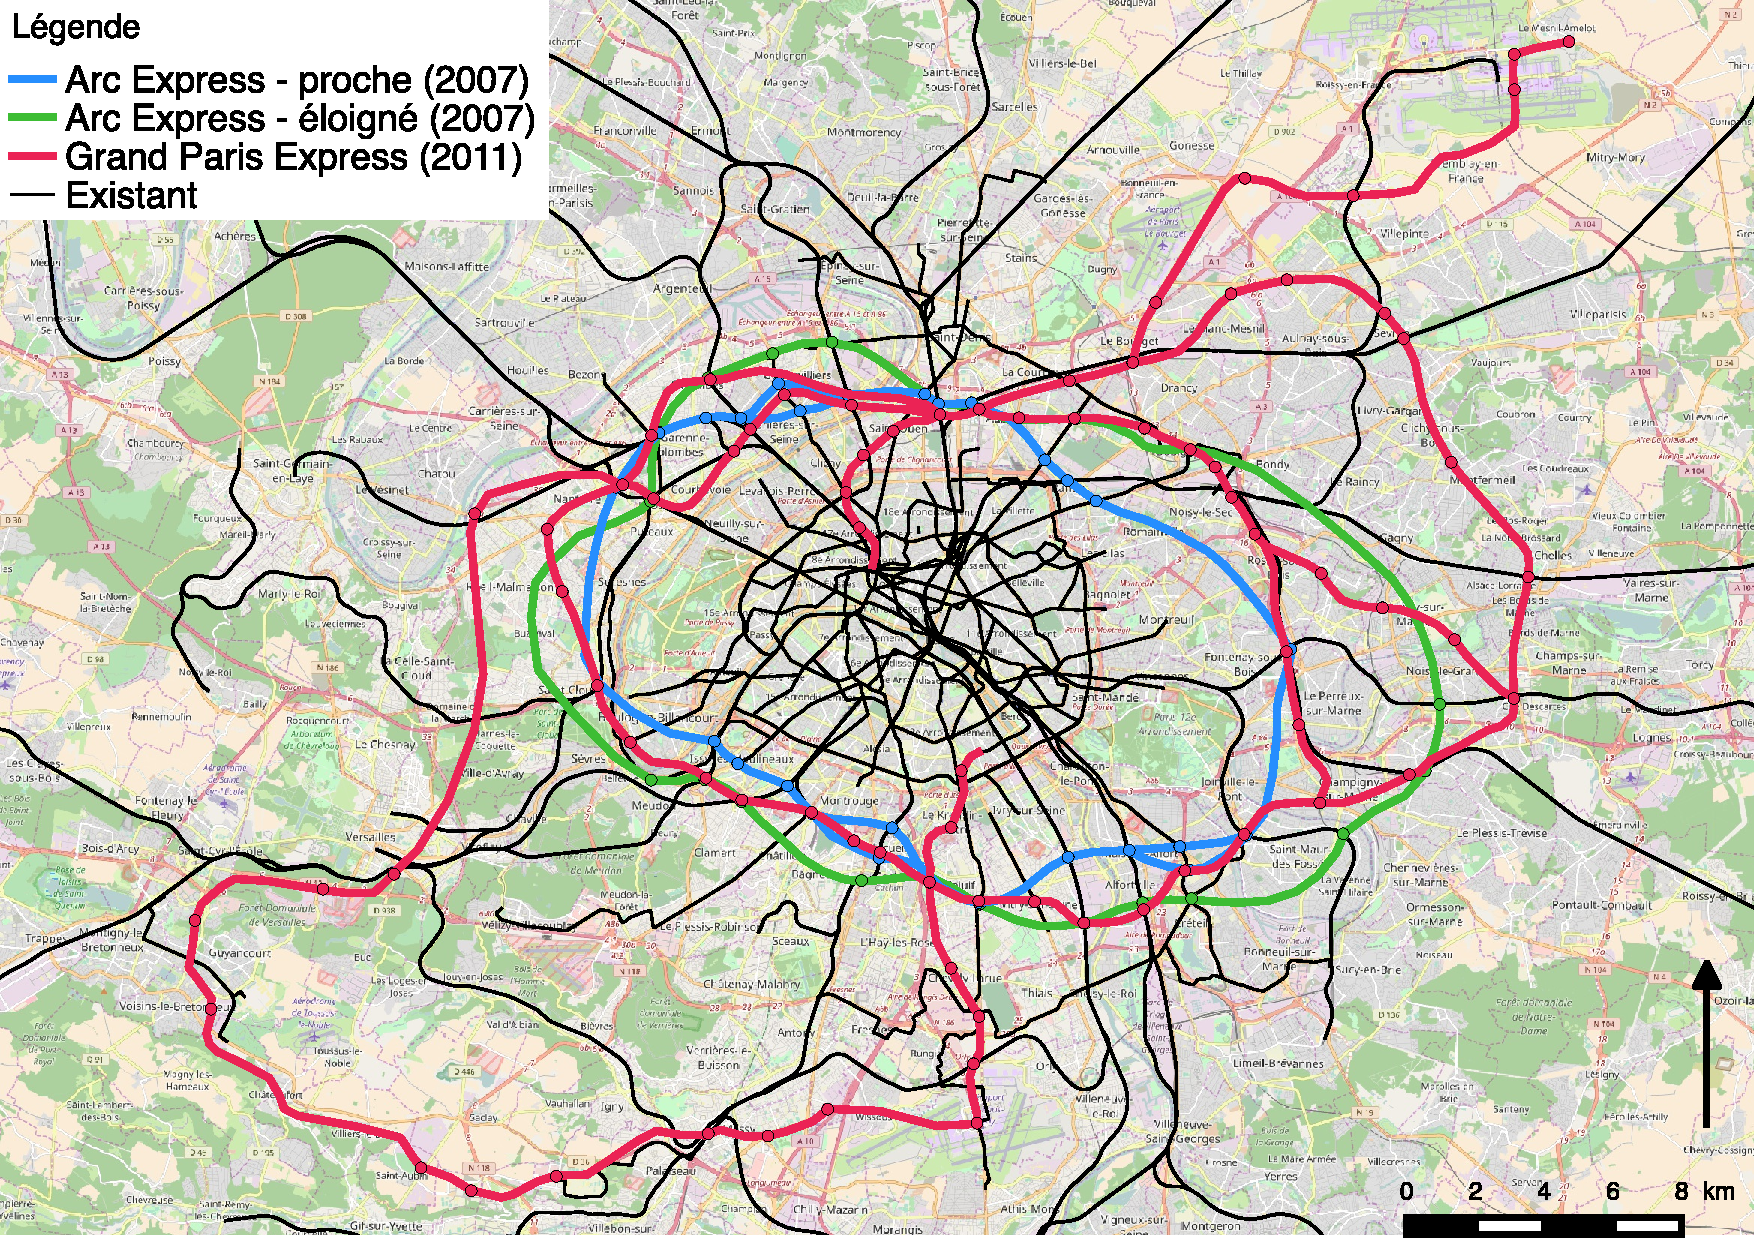
\includegraphics[width=\linewidth]{Figures/GrandParisRealEstate/reseaux}
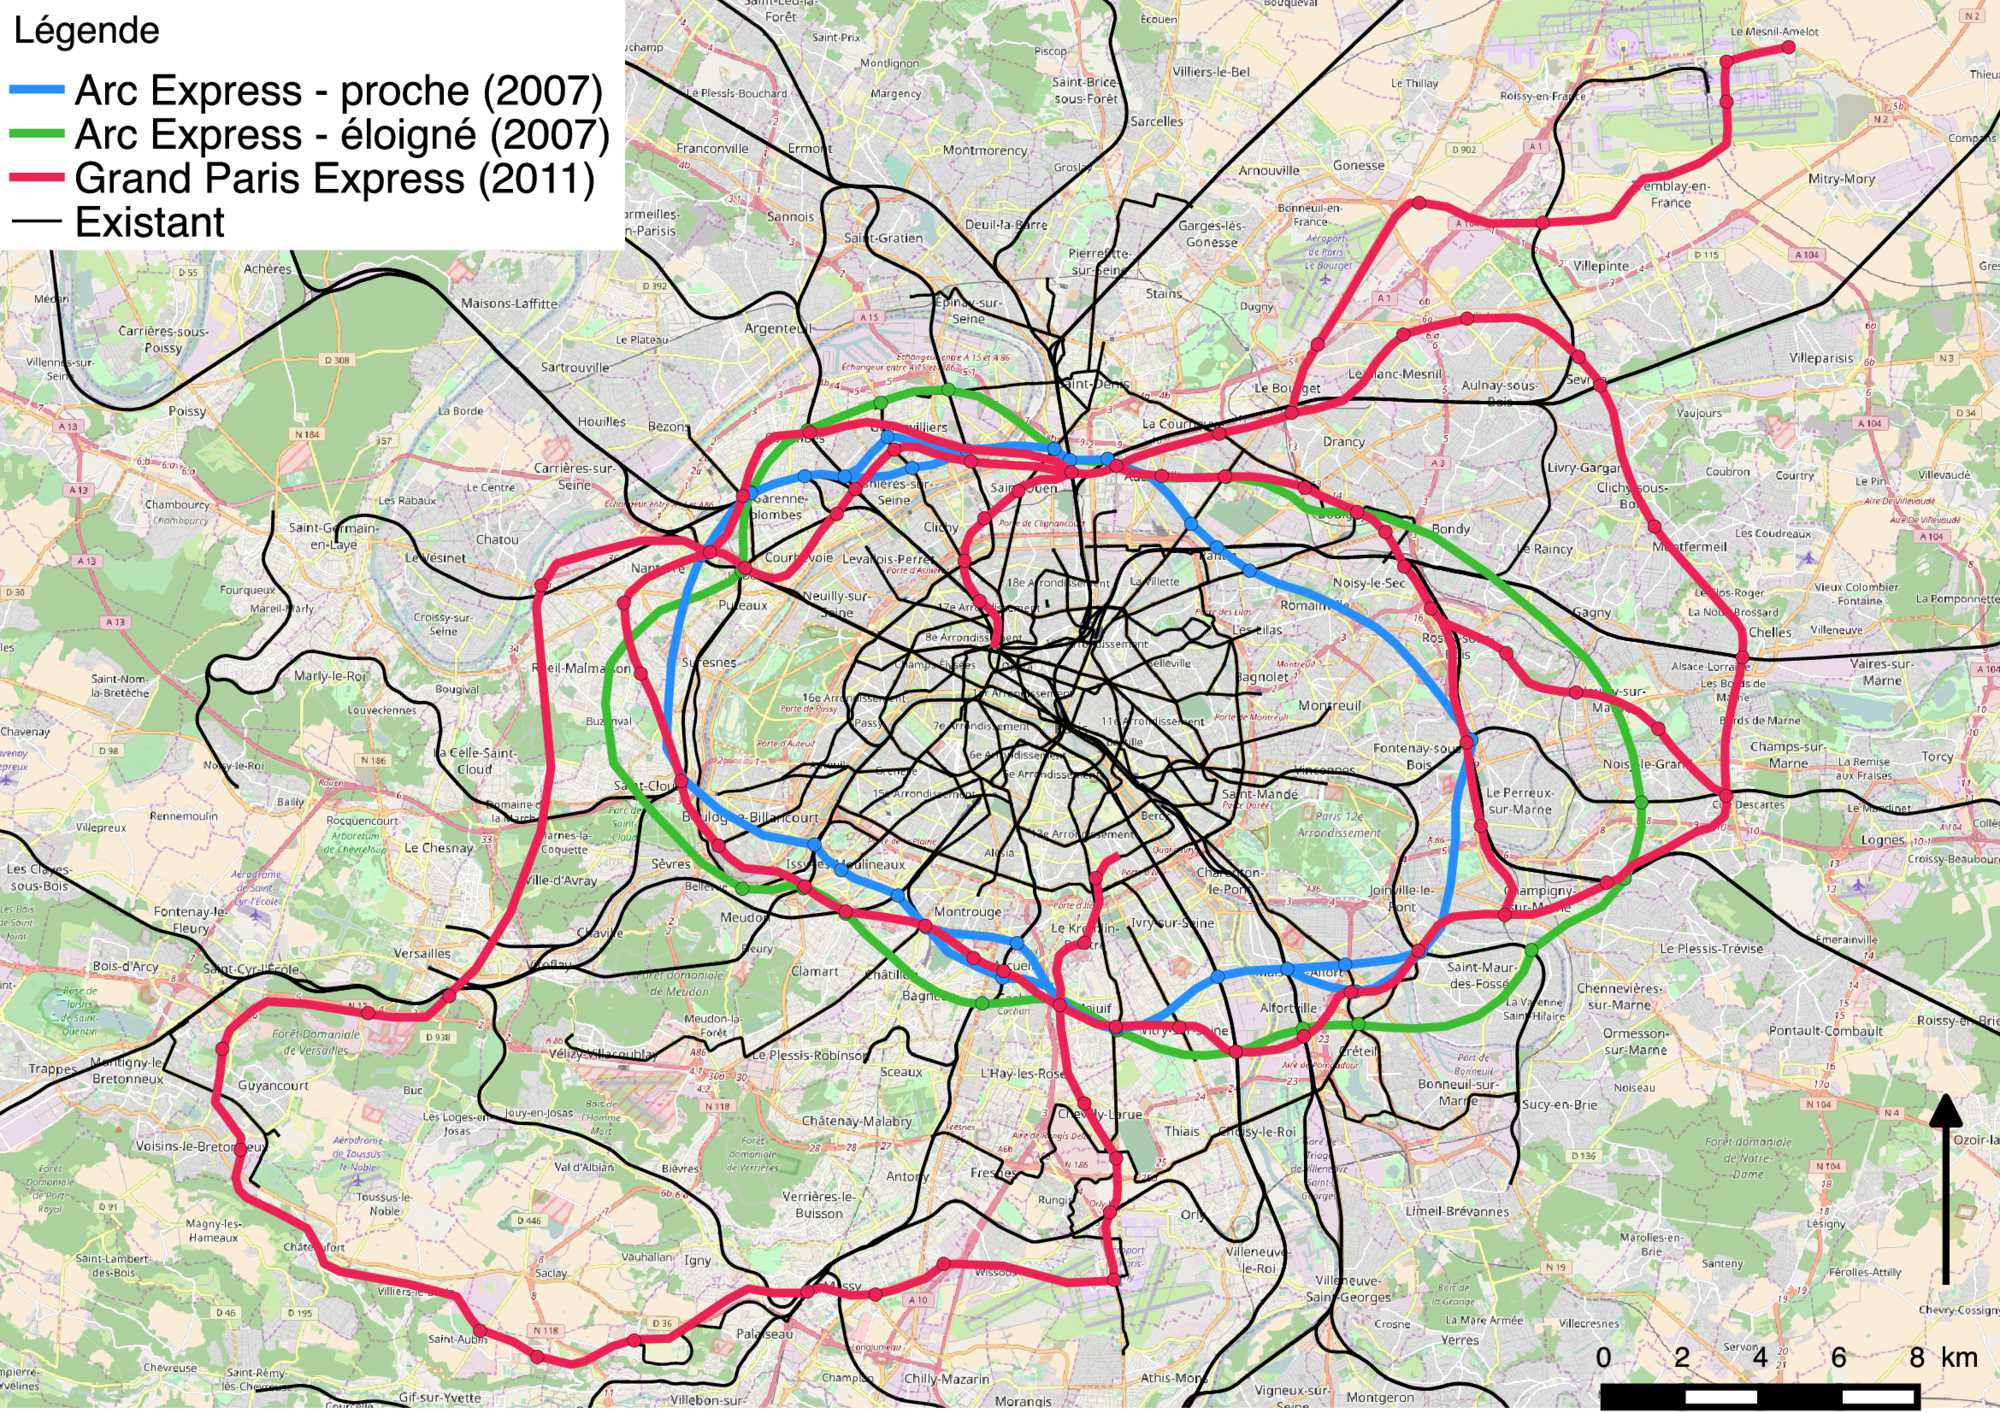
\includegraphics[width=\linewidth]{Figures/Final/1-2-1-fig-casestudies-projects.jpg}
\caption[Successive transportation projects for Greater Paris][Projets de transport successifs du Grand Paris]{\textbf{Successive transportation network projects for the Grand Paris metropolitan area.} We show the two alternatives for the \emph{Arc Express} project elaborated by the Region, and the \emph{Grand Paris Express} (GPE) advocated by the State. The \emph{Réseau du Grand Paris}, a precursor for GPE, is not shown here for visibility reasons because of its proximity with it. The source of the map background, given to situate the lines, is OpenStreetMap.\label{fig:casestudies:projects}}{\textbf{Projets de transport successifs de la métropole du Grand Paris.} Nous montrons les deux alternatives du projet Arc Express porté par la région, et le Grand Paris Express (GPE) porté par l'état, et dont le tracé final résulte d'un compromis entre l'état et la région. Le Réseau du Grand Paris, précurseur du GPE, n'est pas montré ici pour des raisons de visibilité à cause de sa proximité avec celui-ci. Le fond de carte, donné pour indication, a pour source OpenStreetMap.\label{fig:casestudies:projects}}
\end{figure}
%%%%%%%%%%%%%%%



%%%%%%%%%%%%%%%%%%%
\begin{figure}%[h!]
	%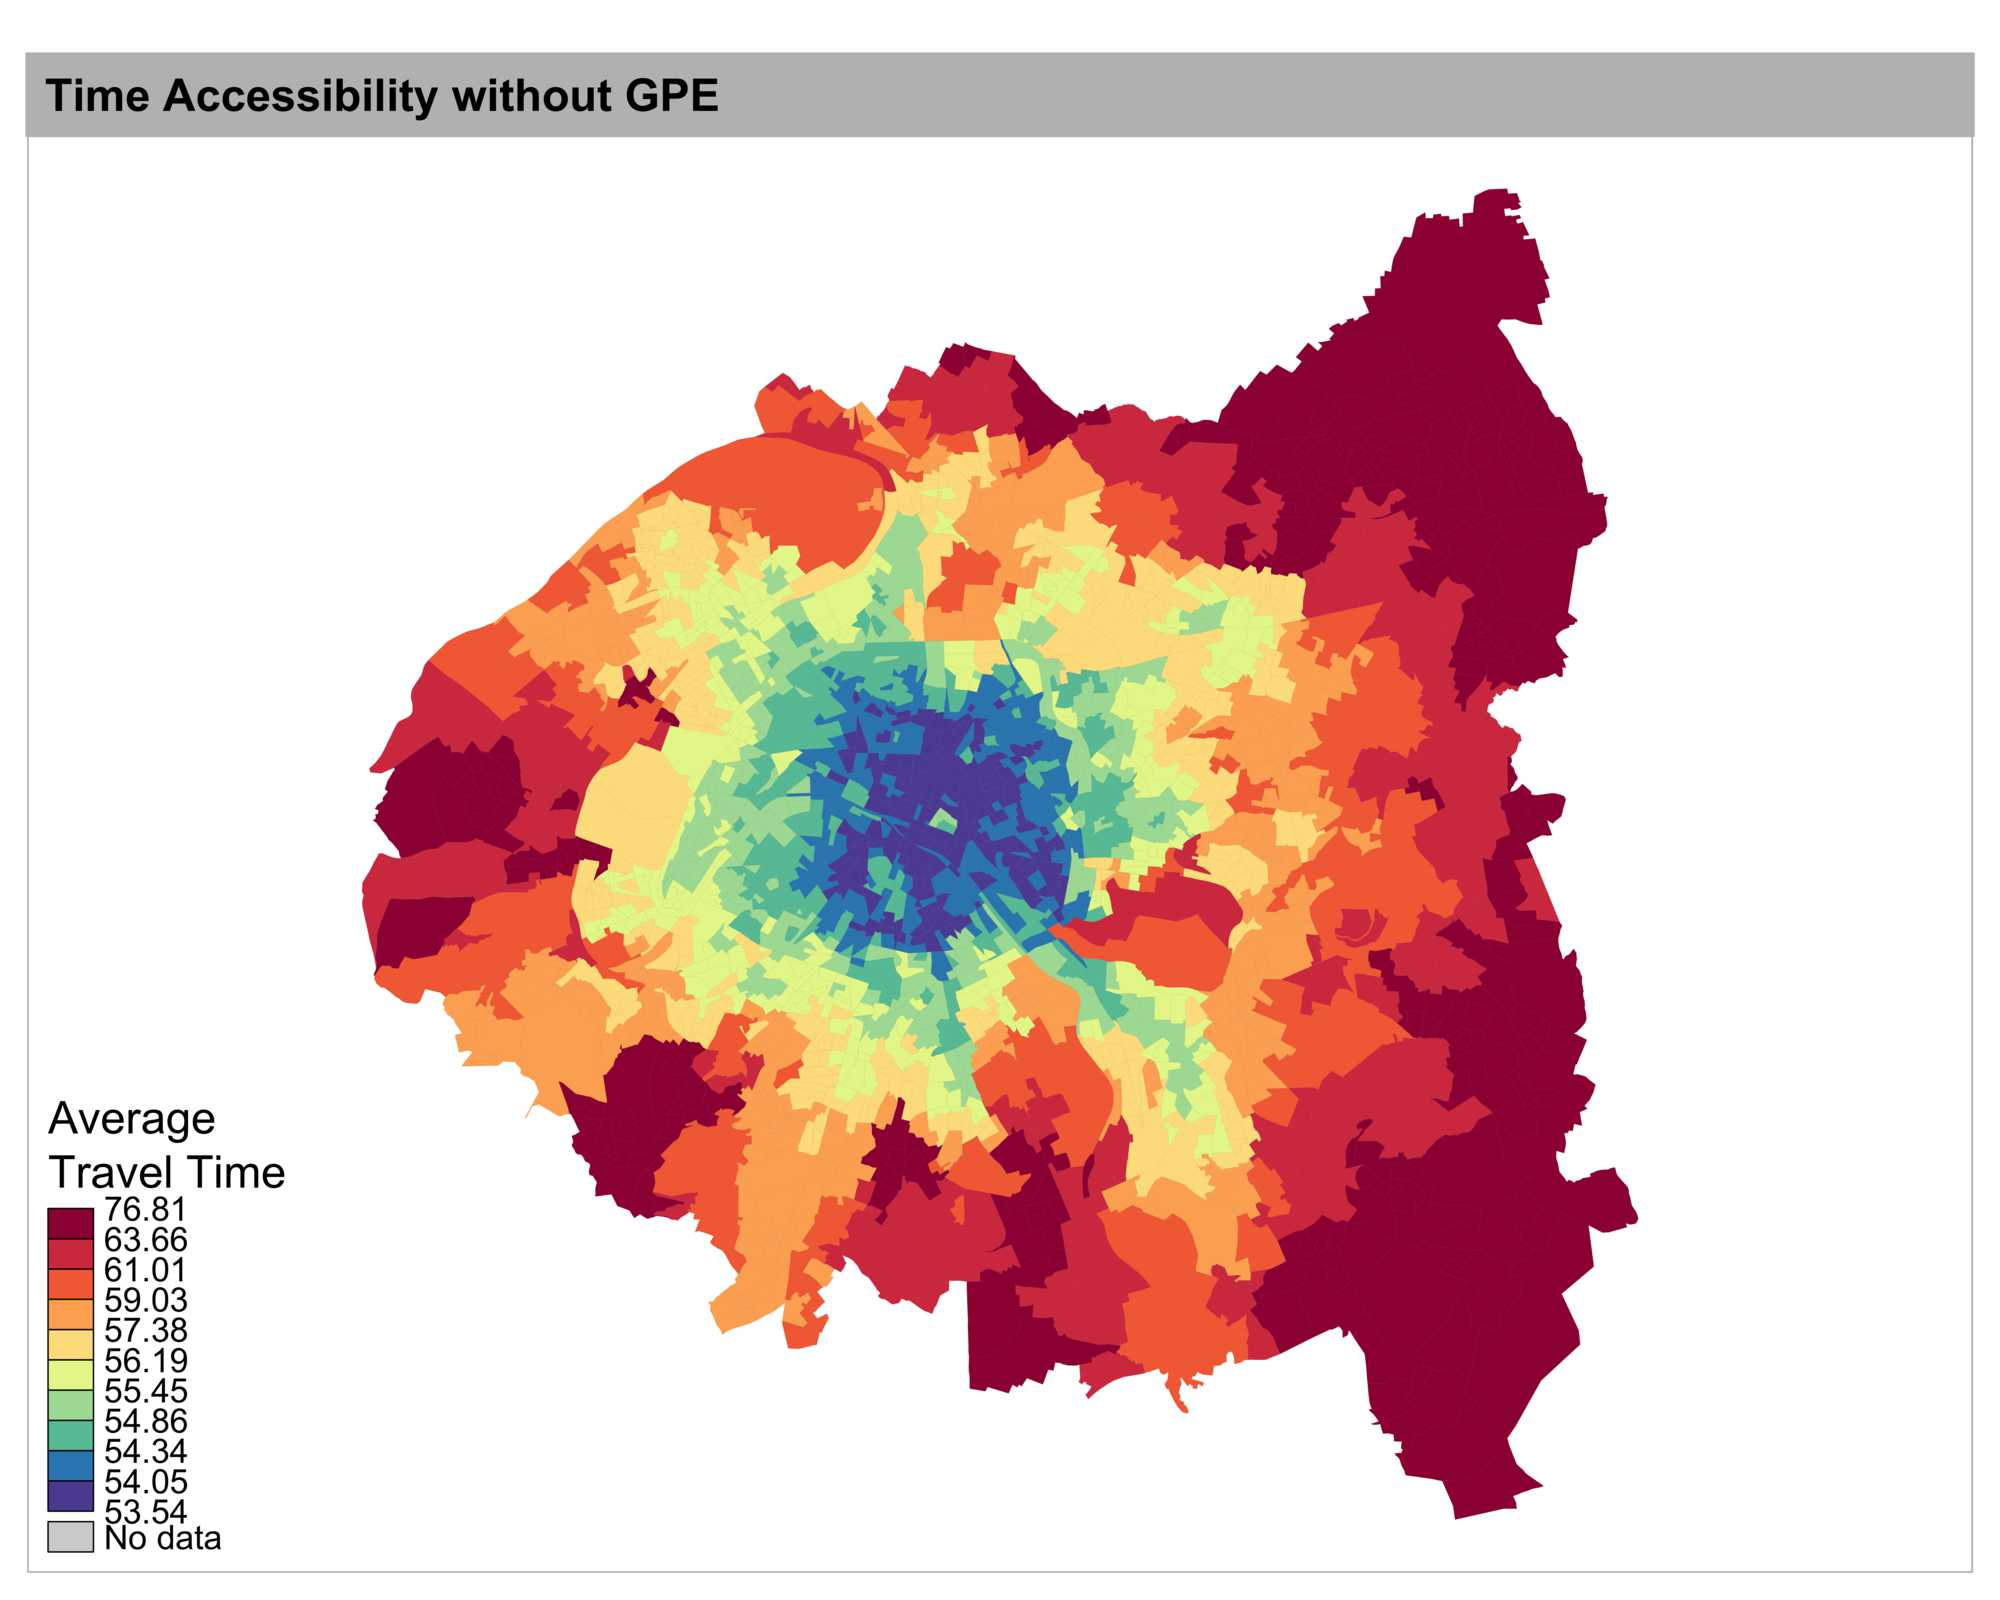
\includegraphics[width=0.8\linewidth]{Figures/CaseStudies/timeaccess_metropole}\\
	%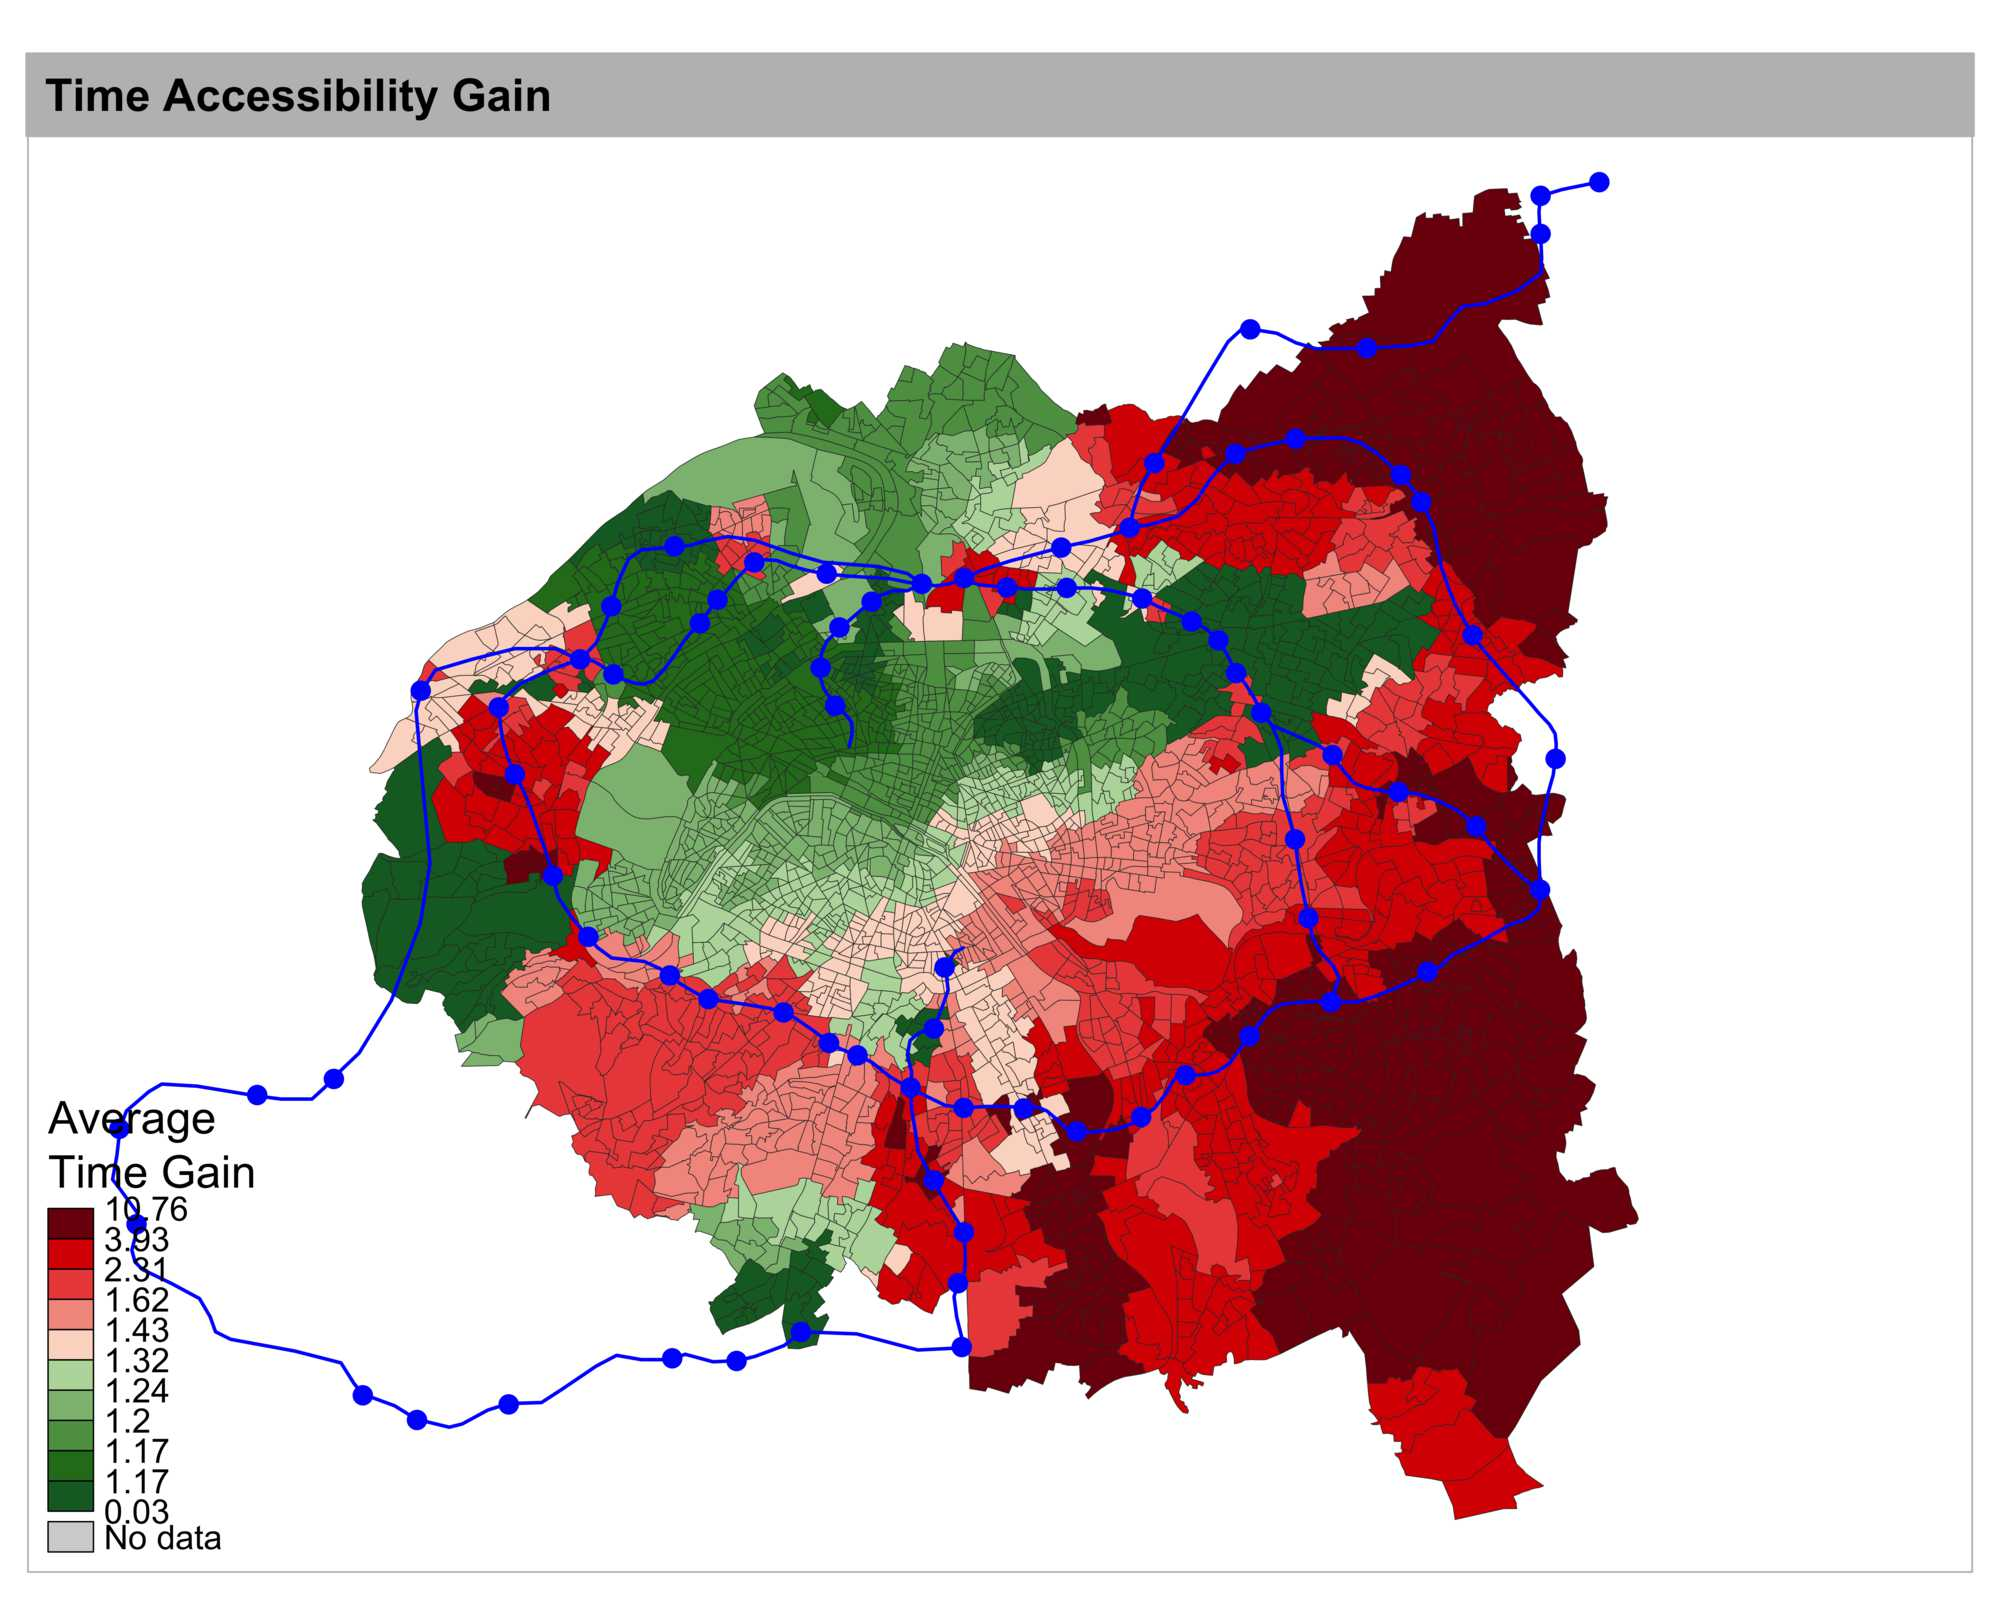
\includegraphics[width=0.8\linewidth]{Figures/CaseStudies/timegain_metropole}
	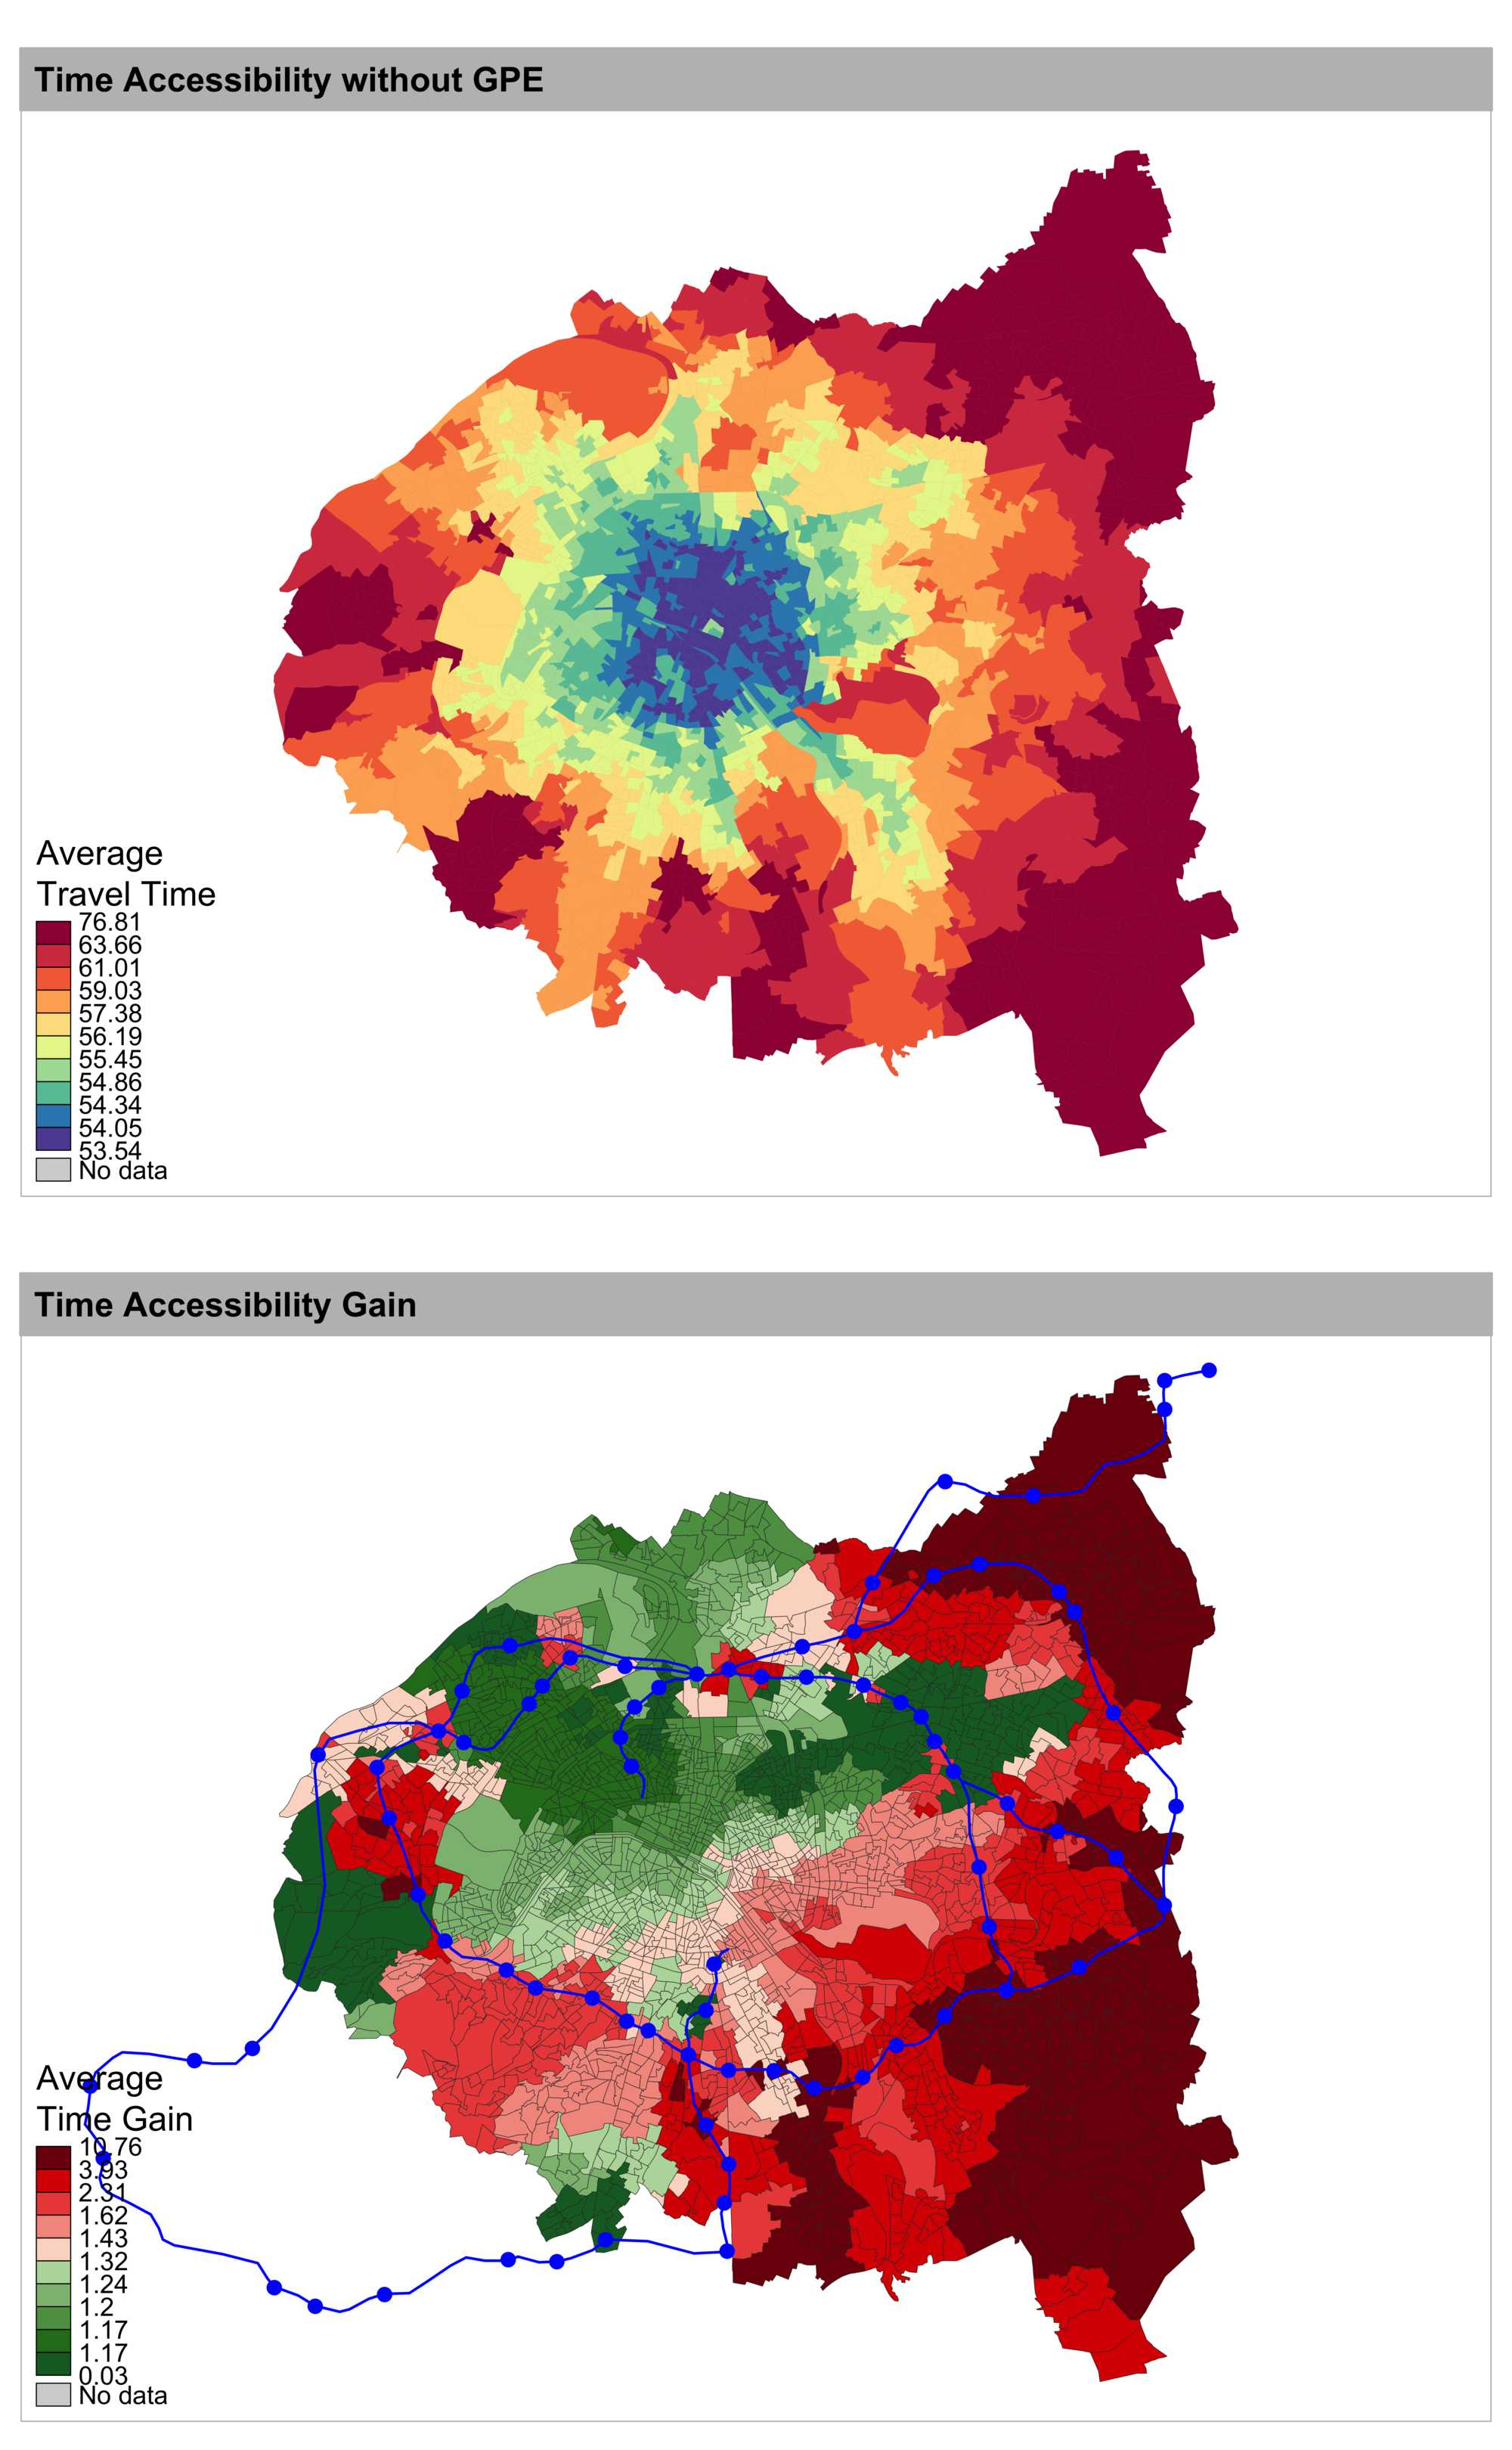
\includegraphics[width=\linewidth]{Figures/Final/1-2-1-fig-casestudies-gpe.jpg}
	\caption[Impact of \emph{Grand Paris Express} on accessibility][Impact du Grand Paris Express sur l'accessibilité]{\textbf{Impact of GPE lines on temporal accessibility.} The map gives, for the \emph{départements de petite couronne} and Paris (75, 92, 93, 94) the temporal accessibility gains, defined for each Iris (elementary infra-communal statistical unit) as the average travel time with public transport to all centroids of other communes, weighted by destination population. The gain is computed as the accessibility difference with and without \emph{Grand Paris Express}. We show a normalized gain, i.e. centered (with a null average) and reduced (unit standard deviation). In blue, the lines and new stations of GPE. We observe the strongest gains mostly in the East, in consistence with the existing literature such as~\cite{beaucire2013grand}. The territorial imprints of RER lines (A in the West, D and B in North, B in the South) exhibit relatively low gains since they are already very accessible.\label{fig:casestudies:gpe}}{\textbf{Impact des lignes du GPE sur l'accessibilité temporelle.} La carte donne, pour les département de la petite couronne et Paris (75, 92, 93, 94) les gains d'accessibilité temporelle, définie pour chaque Iris (unité statistique infra-communale élémentaire) comme le temps moyen de trajet en transport en commun vers l'ensemble des centroïdes des autres communes pondéré par la population de destination. Le gain est calculé comme la différence d'accessibilité avec et sans Grand Paris Express. Nous montrons le gain normalisé, c'est-à-dire centré (de moyenne nulle) et réduit (écart-type unitaire). En bleu, les lignes et nouvelles gare du GPE. On observe les gains les plus forts majoritairement à l'Est, en cohérence avec la littérature existante comme~\cite{beaucire2013grand}. Les sillons territoriaux des lignes de RER (A à l'ouest, D et B au nord, B au sud) présentent des gains relativement faibles car déjà très accessibles.\label{fig:casestudies:gpe}}
\end{figure}
%%%%%%%%%%%%%%%%%%%



\bpar{
The metropolitan region of Paris is currently undergoing significant transformations, with the constitution of a metropolitan governance and new transportation infrastructures. The construction of a ring metro network allowing suburbs to suburbs links answers to an ancient need, and lead to several proposals on which the State and the Region have been in conflict around 2010~\cite{desjardins2010bataille}. The \emph{Arc Express} project~\cite{stif2007arc}, advocated by the Region and more focused on territorial equity, can be contrasted with initial proposals for a \emph{Réseau du Grand Paris} aimed at linking ``excellence clusters'' despite a potential tunnel effect. The solution finally adopted (see the last \emph{Schéma Directeur}~\cite{sdrif2013}) is a compromise and allows a rebalancing of accessibility between the west and the east~\cite{beaucire2013grand}. The Fig.~\ref{fig:casestudies:projects} maps the different projects.
}{
La région métropolitaine de Paris est en train de connaître de grandes mutations, avec la mise en place d'une gouvernance métropolitaine et de nouvelles infrastructures de transport. La construction d'un réseau de métro en rocade permettant des liaisons de banlieue à banlieue répond à un besoin ancien, et a mené à plusieurs propositions sur lesquelles se sont opposés l'Etat et la Région au tournant des années 2010~\cite{desjardins2010bataille}. Le projet Arc Express~\cite{stif2007arc}, porté par la Région et plus axé sur une égalité des territoires, contrastait avec les propositions initiales de Réseau du Grand Paris visant à relier des ``clusters d'excellence'' en dépit d'un possible effet tunnel. La solution finalement adoptée (voir le dernier schéma directeur \cite{sdrif2013}) est un compromis et permet un rééquilibrage est-ouest de l'accessibilité~\cite{beaucire2013grand}. La Fig.~\ref{fig:casestudies:projects} cartographie les différents projets.
}

% Les impacts immédiats d'une nouvelle de transport en terme d'accessibilité concernent généralement des territoires bien plus larges que les zones où la ligne et ses stations sont implantées : les motifs d'accessibilité sont dus aux propriétés topologiques du réseau et celles-ci sont fortement discontinues en fonction de la structure du graphe. Illustrons le cas des lignes du Grand Paris Express et de leur impact direct sur l'accessibilité régionale. La Fig.~\ref{fig:casestudies:accessibility} cartographie pour les départements de la métropole les motifs d'accessibilité et leur évolution directement induite par la construction des nouvelles lignes du Grand Paris.
% %%%%%%%%%%%%%%%%%%%%%%%%
%\begin{figure}
%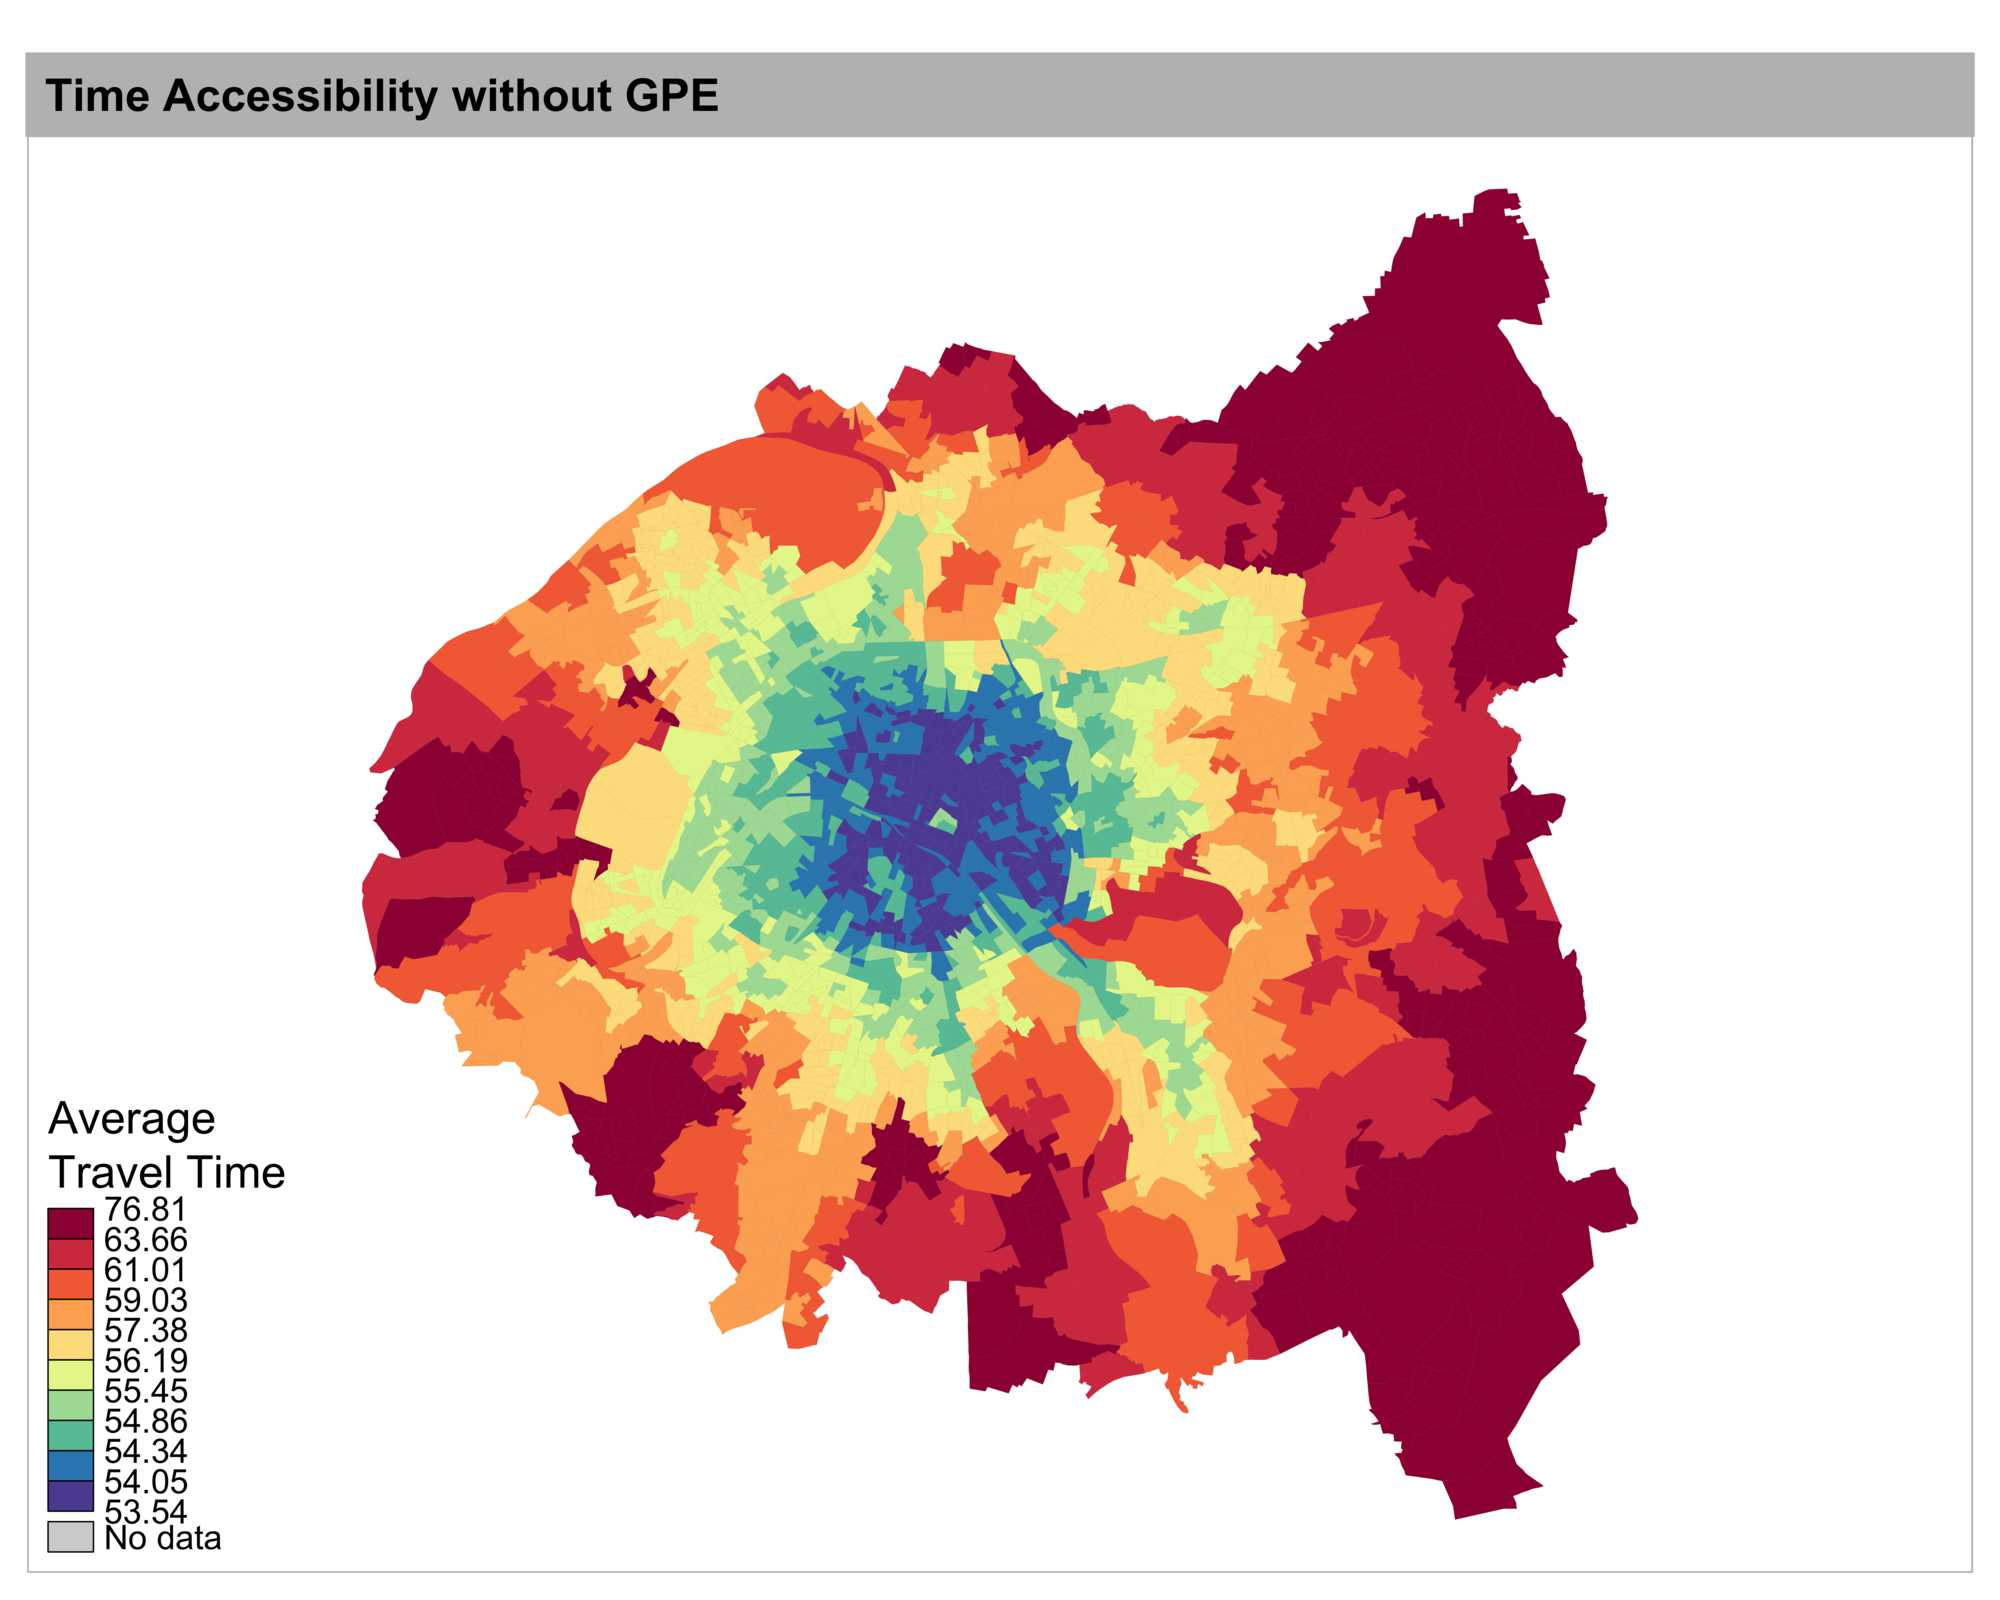
\includegraphics[width=\linewidth]{Figures/CaseStudies/timeaccess_metropole}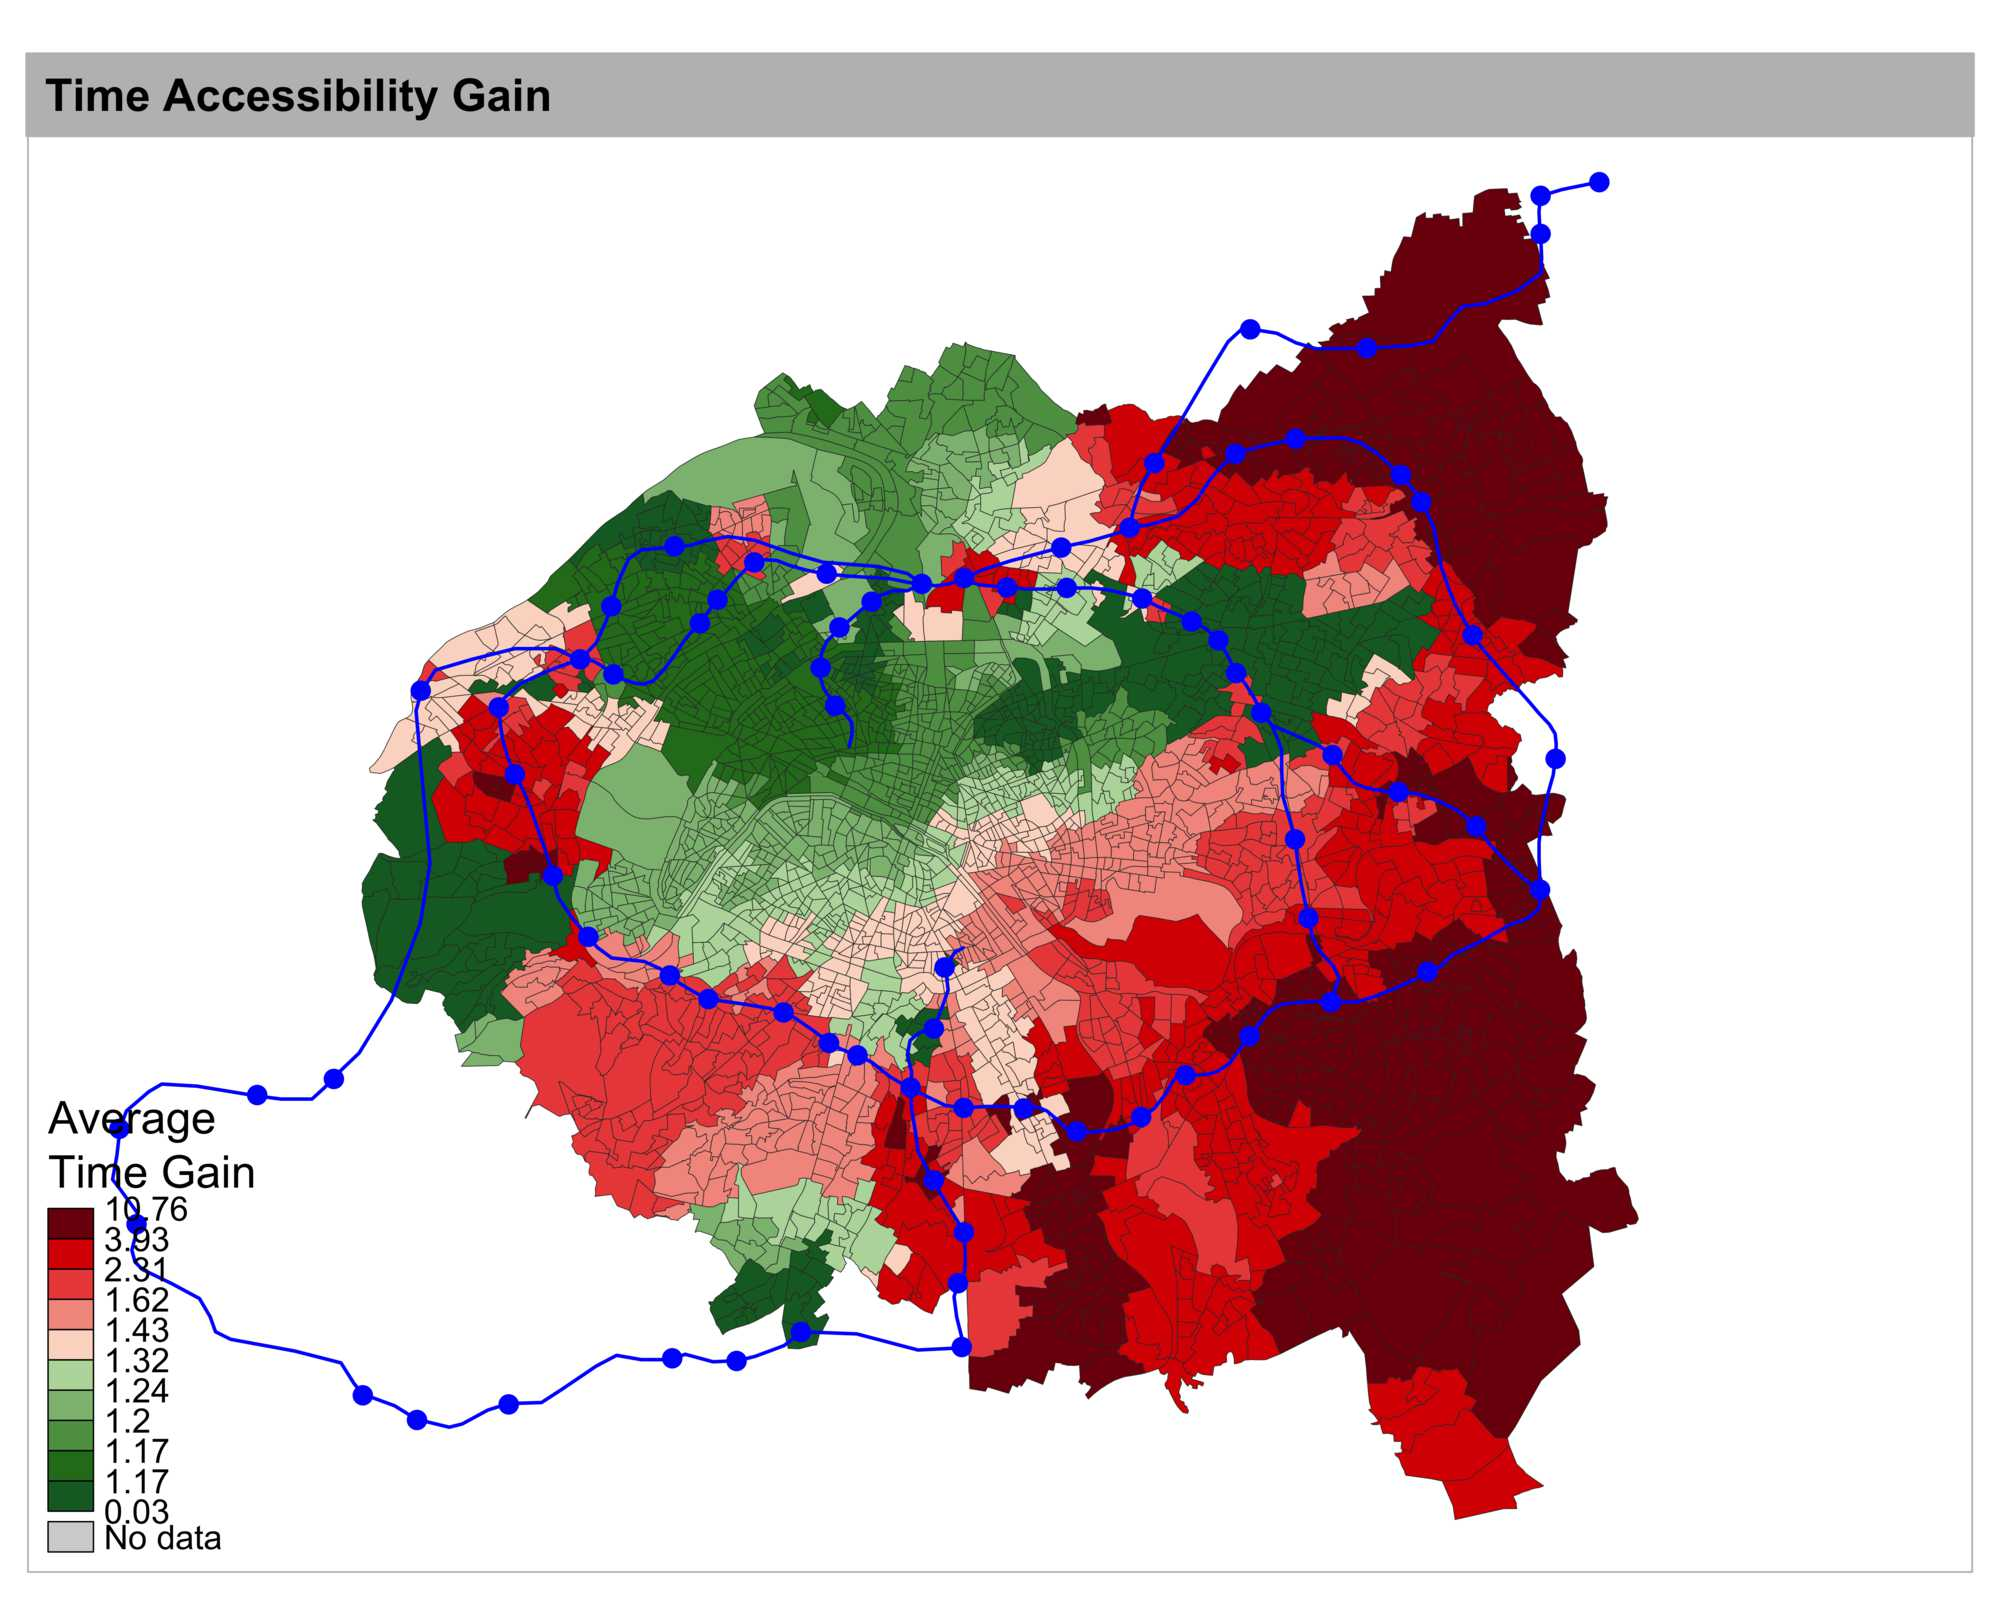
\includegraphics[width=\linewidth]{Figures/CaseStudies/timegain_metropole}
%\caption[Grand Paris Express][Grand Paris Express]{\textbf{Grand Paris Express lines and Accessibility.}}{\textbf{Nouvelles lignes du Grand Paris Express et Accessibilité.} \textit{(Haut)} Accessibilité courantes par Iris, en temps de trajet moyen. \textit{(Bas)} Gain temporels d'accessibilité induits par la réalisation de l'ensemble du projet du Grand Paris Express. \label{fig:casestudies:accessibility}}
%\end{figure}
%%%%%%%%%%%%%%%%%%%%%%%%%


\bpar{
The immediate impacts of a new transportation infrastructure in terms of accessibility, i.e. of the transformation of the spatial distribution of different accessibilities, generally occur for much larger territories than the areas in which the line and its stations are constructed: accessibility patterns are a consequence of topological properties of the network and these are strongly discontinuous as a function of graph structure. We can illustrate the case of \emph{Grand Paris Express} lines and of their direct impact on regional accessibility. We map in Fig.~\ref{fig:casestudies:gpe} the temporal accessibility gains allowed by the \emph{Grand Paris Express} for metropolitan \emph{départements} (75, 92, 93 and 94). The temporal accessibility is computed for each Iris $i$ the following way: with $P_j$ the populations of \emph{communes}, $t_0$ a parameter giving the typical commuting duration (that we fix at one hour~\cite{zahavi1980regularities}), $t_{ij}$ the travel time with public transport between the centroid of $i$ and the one of commune $j$, we take a weighted average defined by
}{
Les impacts immédiats d'une nouvelle infrastructure de transport en termes d'accessibilité, c'est-à-dire la transformation de la distribution spatiale des différentes accessibilités, concernent généralement des territoires bien plus larges que les zones où la ligne et ses stations sont implantées : les motifs d'accessibilité sont dus aux propriétés topologiques du réseau et celles-ci sont fortement discontinues en fonction de la structure du graphe. Illustrons le cas des lignes du Grand Paris Express et de leur impact direct sur l'accessibilité régionale. Nous cartographions en Fig.~\ref{fig:casestudies:gpe} les gains d'accessibilité temporelle permis par le projet du Grand Paris Express sur les départements métropolitains (75, 92, 93 et 94). L'accessibilité temporelle est calculée pour chaque Iris $i$ de la manière suivante : avec les populations des communes $P_j$, $t_0$ un paramètre de durée typique d'un déplacement (que nous fixons à une heure~\cite{zahavi1980regularities}), $t_{ij}$ le temps de trajet en transports en commun entre le centroïde de $i$ et celui de la commune $j$, nous prenons une moyenne pondérée définie comme
}

\[
Z_i = \sum_j \left(\frac{P_j}{\sum_k P_k}\right)\cdot \exp\left(- t_{ij}/t_0\right)
\]


\bpar{
This expression indeed allows to have an accessibility potential, and the weighting be population should remove some bias due to potentially negligible trajectories as a proportion of total travels. We recall that this is a normative accessibility in the sense of \cite{paez2012measuring} since the gravity parameter is fixed in a stylized way.
}{
Cette expression permet de bien avoir un potentiel d'accessibilité, et la pondération par la population permet de ne pas biaiser l'indicateur par des trajets potentiellement négligeables en proportion des trajets totaux. Notons qu'il s'agit d'une accessibilité normative au sens de \cite{paez2012measuring} puisque le paramètre gravitaire est fixé de manière stylisée.
}



\bpar{
We observe, in accordance with the analysis by~\cite{beaucire2013grand}, a rebalancing of accessibility differentials between the East and the West. At an equal distance of the center, accessibility is lower for Seine-Saint-Denis and Val-de-Marne that for Hauts-de-Seine, i.e. that these \emph{départements} have potentially more difficulties to access the rest of the metropolis. The map of average time gains also exhibits the highest gains for this two \emph{départements}. Some \emph{communes} that are socially and economically disadvantaged as Aulnay benefit from the highest time gains. The line 16 indeed allows a significant opening up of the North-east of Seine-Saint-Denis~\cite{desjardins2016grand}. The creation of links from suburbs to suburbs is a crucial aspect of this opening up and is conceived as a motor of the emergence of new centralities, towards an always more polycentric metropolis, in the inheritance of the planning policy of \emph{Villes Nouvelles}, in order to obtain not neighboring suburbs anymore but districts that are a full part of Greater Paris. The effects can remain however mitigated depending on the areas: \cite{l2013grand} show that the \emph{Grand Paris Express} will induce a direct access to a larger number of employments for a significant number of unemployed within the \emph{Petite Couronne}, but that inequalities with \emph{Grande Couronne} will increase and that there exists some risks of dropping out for far away \emph{communes} with a low accessibility.
}{
Nous observons, conformément à l'analyse de~\cite{beaucire2013grand}, un rééquilibrage des différentiels d'accessibilité entre Est et Ouest. A distance égale du centre, l'accessibilité est plus basse pour la Seine-Saint-Denis et le Val-de-Marne que pour les Hauts-de-Seine, c'est-à-dire que ces départements ont potentiellement plus de difficultés pour accéder au reste de la métropole. La carte des gains temporels moyens montre les gains plus grands également pour ces deux départements. Des communes socio-économiquement défavorisées comme Aulnay sont bénéficiaires des plus grands gains de temps. La ligne 16 permet en effet un désenclavement significatif du nord-est de la Seine-Saint-Denis~\cite{desjardins2016grand}. La création de liaisons de banlieue à banlieue est un aspect majeur de ce désenclavement et est voulue comme un moteur de l'émergence de nouvelles centralités, vers une métropole toujours plus polycentrique, dans la lignée de la politique d'aménagement des villes nouvelles, pour ne plus parler de proche banlieue mais de quartiers faisant partie intégrante du Grand Paris. Les effets peuvent cependant être mitigés selon les zones : \cite{l2013grand} montrent que le Grand Paris Express induira un accès direct à un plus grand nombre d'emplois pour un nombre significatif de chômeurs en petite couronne, mais que les écarts avec la grande couronne seront accentués et qu'il existe des risques de décrochage de certaines communes lointaines mal desservies.
}


\bpar{
One of the crucial issues for the construction of Greater Paris is to stay careful on not obtaining a metropolis with multiple separated levels, and to exploit the increased connectivity at different scales (international, national, regional, metropolitan) in order to reduce territorial inequalities instead of increasing them\footnote{We recall that an unequal distribution of agents and resources will generate differences in potential larger than a uniform distribution, these can then be linked to the evolution of the network.}. The novel network seems to contribute to this dynamic, under the condition of a coordinated territorial development, allowing the realization of immediate accessibility gains in terms of territorial transformations. There exists no method that can forecast it in a deterministic way as we already developed. It is however possible to retrospectively analyze from an empirical point of view the couplings between territorial variables and network variables, in order to quantitatively unveil co-evolution phenomena. We propose now to illustrate this approach.  
}{
L'un des enjeux cruciaux pour la construction du Grand Paris est de veiller à ne pas obtenir une métropole à plusieurs vitesses, et de tirer parti de la connectivité accrue à plusieurs échelles (internationale, nationale, régionale, métropolitaine) pour réduire les inégalités territoriales plutôt que les accroitre\footnote{Rappelons qu'une inégale répartition des agents et des ressources générera des différences de potentiel plus grandes qu'une distribution uniforme, celles-ci pouvant alors être liées à l'évolution du réseau.}. Le nouveau réseau semble contribuer à cette dynamique, sous condition d'un développement territorial coordonné, permettant la concrétisation des gains immédiats d'accessibilité en terme de transformation territoriale. Il n'existe pas de méthode pouvant prévoir celle-ci de manière déterministe comme nous l'avons déjà développé. Il est cependant possible d'analyser rétrospectivement de manière empirique les couplages entre variables territoriales et variables de réseau, pour essayer de mettre en valeur quantitativement les phénomènes de co-évolution. Nous proposons à présent d'illustrer cette démarche.
}






\subsubsection{Linking territorial dynamics and construction of the Grand Paris Express}{Lier dynamiques territoriales et construction du Grand Paris Express}



\bpar{
One of the aims of our work in the following will be to empirically clarify situations in which strongly coupled dynamics linked to our problematic can be exhibited, and then through models to isolate processes and conditions allowing one or the other situation. We propose to deepen the illustration of GPE, while introducing a potential approach to link a territorial dynamic with the one of the anticipated network.
}{
L'un des enjeux de notre travail par la suite sera de clarifier empiriquement des situations dans lesquelles des dynamiques fortement couplées relevant de cette problématique pourront être mises en évidence, puis à travers des modèles d'isoler des processus et des conditions permettant telle ou telle situation. Nous proposons d'approfondir l'illustration du GPE, tout en introduisant une approche possible pour lier dynamique territoriale et celle du nouveau réseau anticipé.
}


\bpar{
Various aspects of territories are concerned by interactions with networks. In previous empirical studies, no socio-economic attributes of populations inhabiting the territory nor economic values for land and real estate was considered. Both are however crucial elements of territorial dynamics and are extensively studied in fields such as territorial analysis or urban economics : for example, \cite{homocianu:tel-00359302} studies households residential choices to understand land-use transportation interactions. We propose here to use a database of Real Estate transactions for Parisian region on the last 20 years, with 2 years temporal granularity and exact spatial coordinates. \cite{guerois2009dynamique} used it for example to obtain typologies of spatial dynamics of the Parisian real estate market.
}{
Des aspects très variés des territoires sont concernés par l'interaction avec les réseaux. Dans nos études précédentes, les aspects économiques et financiers du foncier et l'immobilier n'ont pas été considérés. Il s'agit cependant d'éléments cruciaux des dynamiques territoriales et sont étudiés de manière intensive dans des champs comme l'analyse territoriale ou l'économie urbaine : par exemple, \cite{homocianu:tel-00359302} étudie les choix résidentiels des ménages pour comprendre les interactions entre usage du sol et transport. Nous proposons ici d'utiliser entre autres une base de données de transactions immobilières pour la région parisienne sur les 20 dernières années, avec une granularité temporelle de 2 ans et coordonnées spatiales exactes. \cite{guerois2009dynamique} l'utilise par exemple pour établir une typologie des dynamiques spatiales du marché immobilier parisien.
}



\bpar{
This more precise study can be understood as a research of early warnings of network potential breakdowns: indeed, if intrinsic territorial dynamics anticipate the arrival of a new public transportation station, the implications will be much different to the case where it will then drive these variables after its construction. The interpretation in terms of ``structuring effects'' will indeed be significantly different. We apply here the method of spatio-temporal causalities developed in~\ref{sec:causalityregimes}. We propose to study the relations between the accessibility differential for each project, and variables linked to land (real estate transactions) and socio-economical, in order to see if it is possible to capture a link between accessibility differentials and differentials in territorial variables. Indeed, the links between new lines and real estate value evolution are sometimes dramatic~\cite{damm1980response}. 
}{
Cette étude plus précise peut être comprise comme une recherche de signes précurseurs de rupture de potentiels du réseau : en effet, si des dynamiques territoriales intrinsèques anticipent l'arrivée d'une nouvelle station de transports en commun, les implications seront bien différentes du cas où celle-ci conduit ces variables après sa construction. L'interprétation en termes ``d'effets structurants'' sera notamment très différente. Nous appliquons ici la méthode de causalités spatio-temporelles développée en~\ref{sec:causalityregimes}. Nous proposons d'étudier les relations entre différentiel d'accessibilité pour chaque projet, et variables liées au foncier (transactions immobilières) et socio-économiques, afin de voir s'il est possible de capturer un lien entre les différentiels d'accessibilité et les différentiels des variables territoriales. En effet, les liens entre nouvelles lignes et évolution du foncier sont parfois remarquables~\cite{damm1980response}.
}



%\comment{sur les anticipations des acteurs : \cite{carrouet:hal-00980002} }

%\cite{guerois2009dynamique} : bulles immobilières locales ?


\bpar{
Data for real estate transactions are provided by the BIENS database (\emph{Chambre des Notaires d'Ile de France}, proprietary database). The number of transactions that can be used after cleaning is 862360, distributed across all IRIS areas (basic census units in France), for a temporal span covering the years 2003 to 2012 included. The data at the IRIS level for population and income (median income and Gini index) come from INSEE. Network data have been vectorialized from projects maps (see figure~\ref{fig:projects} for the different projects). Travel times are computed by public transportation only, with standard values for average speeds of different modes\footnote{That we take as the following: RER 60km.h\textsuperscript{-1}, Transilien 100km.h\textsuperscript{-1}, Metro 30km.h\textsuperscript{-1}, Tramway 20km.h\textsuperscript{-1}.}.
}{
Les données des transactions immobilières sont fournies par la base BIENS (Chambre des Notaires d'Ile de France, base propriétaire). Le nombre de transactions utilisables après nettoyage est de 862360, se répartissant sur l'ensemble des IRIS, pour une plage temporelle couvrant de 2003 à 2012 incluses. Les données par IRIS pour population et revenu (revenu médian et indice de Gini) proviennent de l'INSEE. Les données de réseau ont été vectorialisées à partir des cartes des projets (voir Fig.~\ref{fig:casestudies:projects} pour les projets). Les temps de trajets sont calculés par transport en commun uniquement, avec des valeurs standard pour les vitesses moyennes des différents modes~\cite{larroque2002paris}\footnote{Que nous prenons les suivantes : RER 60km.h\textsuperscript{-1}, Transilien 100km.h\textsuperscript{-1}, Metro 30km.h\textsuperscript{-1}, et Tramway 20km.h\textsuperscript{-1}.}.
}

%\begin{table}
%\begin{tabular}{|c|c|}\hline
%	Mode & Vitesse moyenne \\\hline
%	RER & 60km.h\textsuperscript{-1}\\
%	Transilien & 100km.h\textsuperscript{-1}\\
%	Metro & 30km.h\textsuperscript{-1}\\
%	Tramway & 20km.h\textsuperscript{-1}\\\hline
%\end{tabular}
%\end{table}

\bpar{
The travel time matrix is computed from all the centroids of IRIS to all the centroids of \emph{Communes} (above aggregation level). These are linked to the network with abstract connectors to the closest station, with a speed of 50km.h\textsuperscript{-1} (travel by car). Analysis are implemented in R~\cite{R-Core-Team:2015fk} and all data, source code and results are available on an open git repository\footnote{At\\\texttt{https://github.com/JusteRaimbault/CityNetwork/tree/master/Models/SpatioTempCausality/GrandParis}. Data for the BIENS database are given only at the aggregated level of IRIS and for price and mortgage variables, for contractual reasons closing the database.}.
}{
La matrice des temps est calculée depuis l'ensemble des centroïdes des IRIS vers l'ensemble des centroïdes des communes. Ceux-ci sont reliés au réseau par des connecteurs à la gare la plus proche, de vitesse 50km.h\textsuperscript{-1} (trajet en voiture). Les analyses sont implémentées intégralement en langage R~\cite{R-Core-Team:2015fk} et l'ensemble des données, du code source et des résultats sont disponibles sur un dépôt git ouvert\footnote{A l'adresse \url{https://github.com/JusteRaimbault/CityNetwork/tree/master/Models/SpatioTempCausality/GrandParis}. Les données de la base BIENS ne peuvent être fournies pour raison de fermeture contractuelle de la base.}.
}




%%%%%%%%%%%%%%%
\begin{figure}%[h!]
%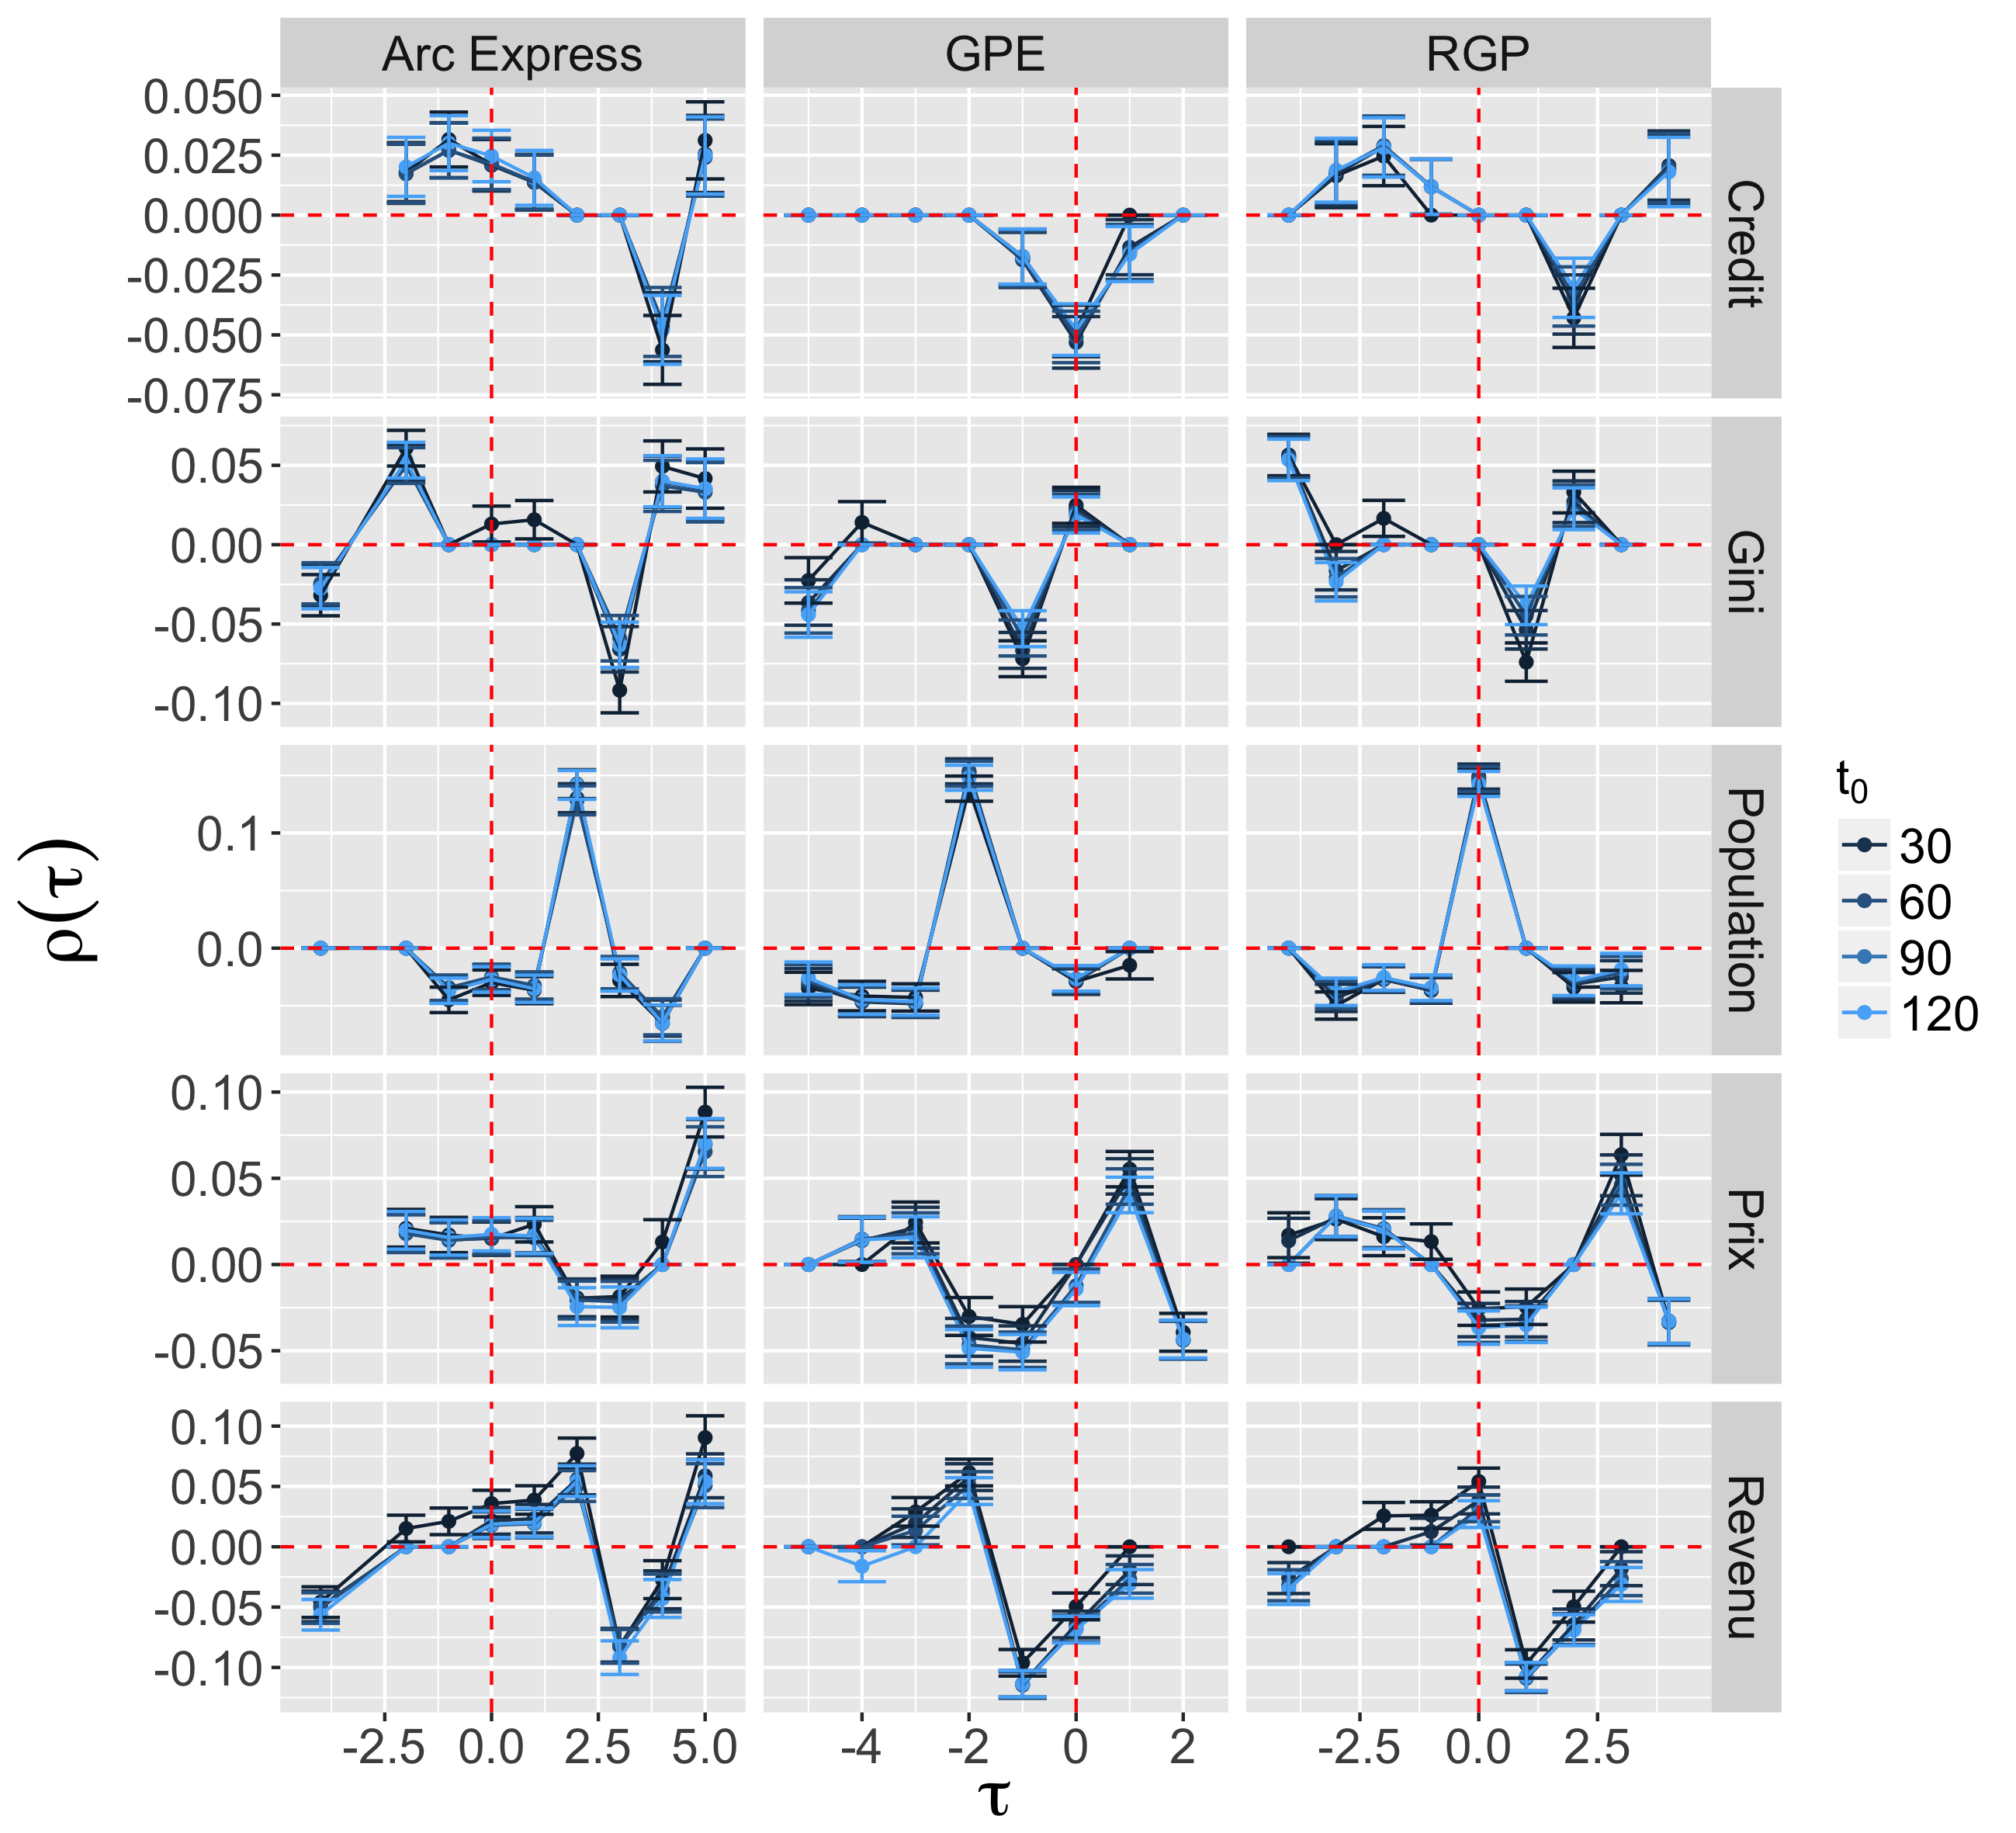
\includegraphics[width=\linewidth]{Figures/GrandParisRealEstate/laggedcorrs_times_allvars_fr}
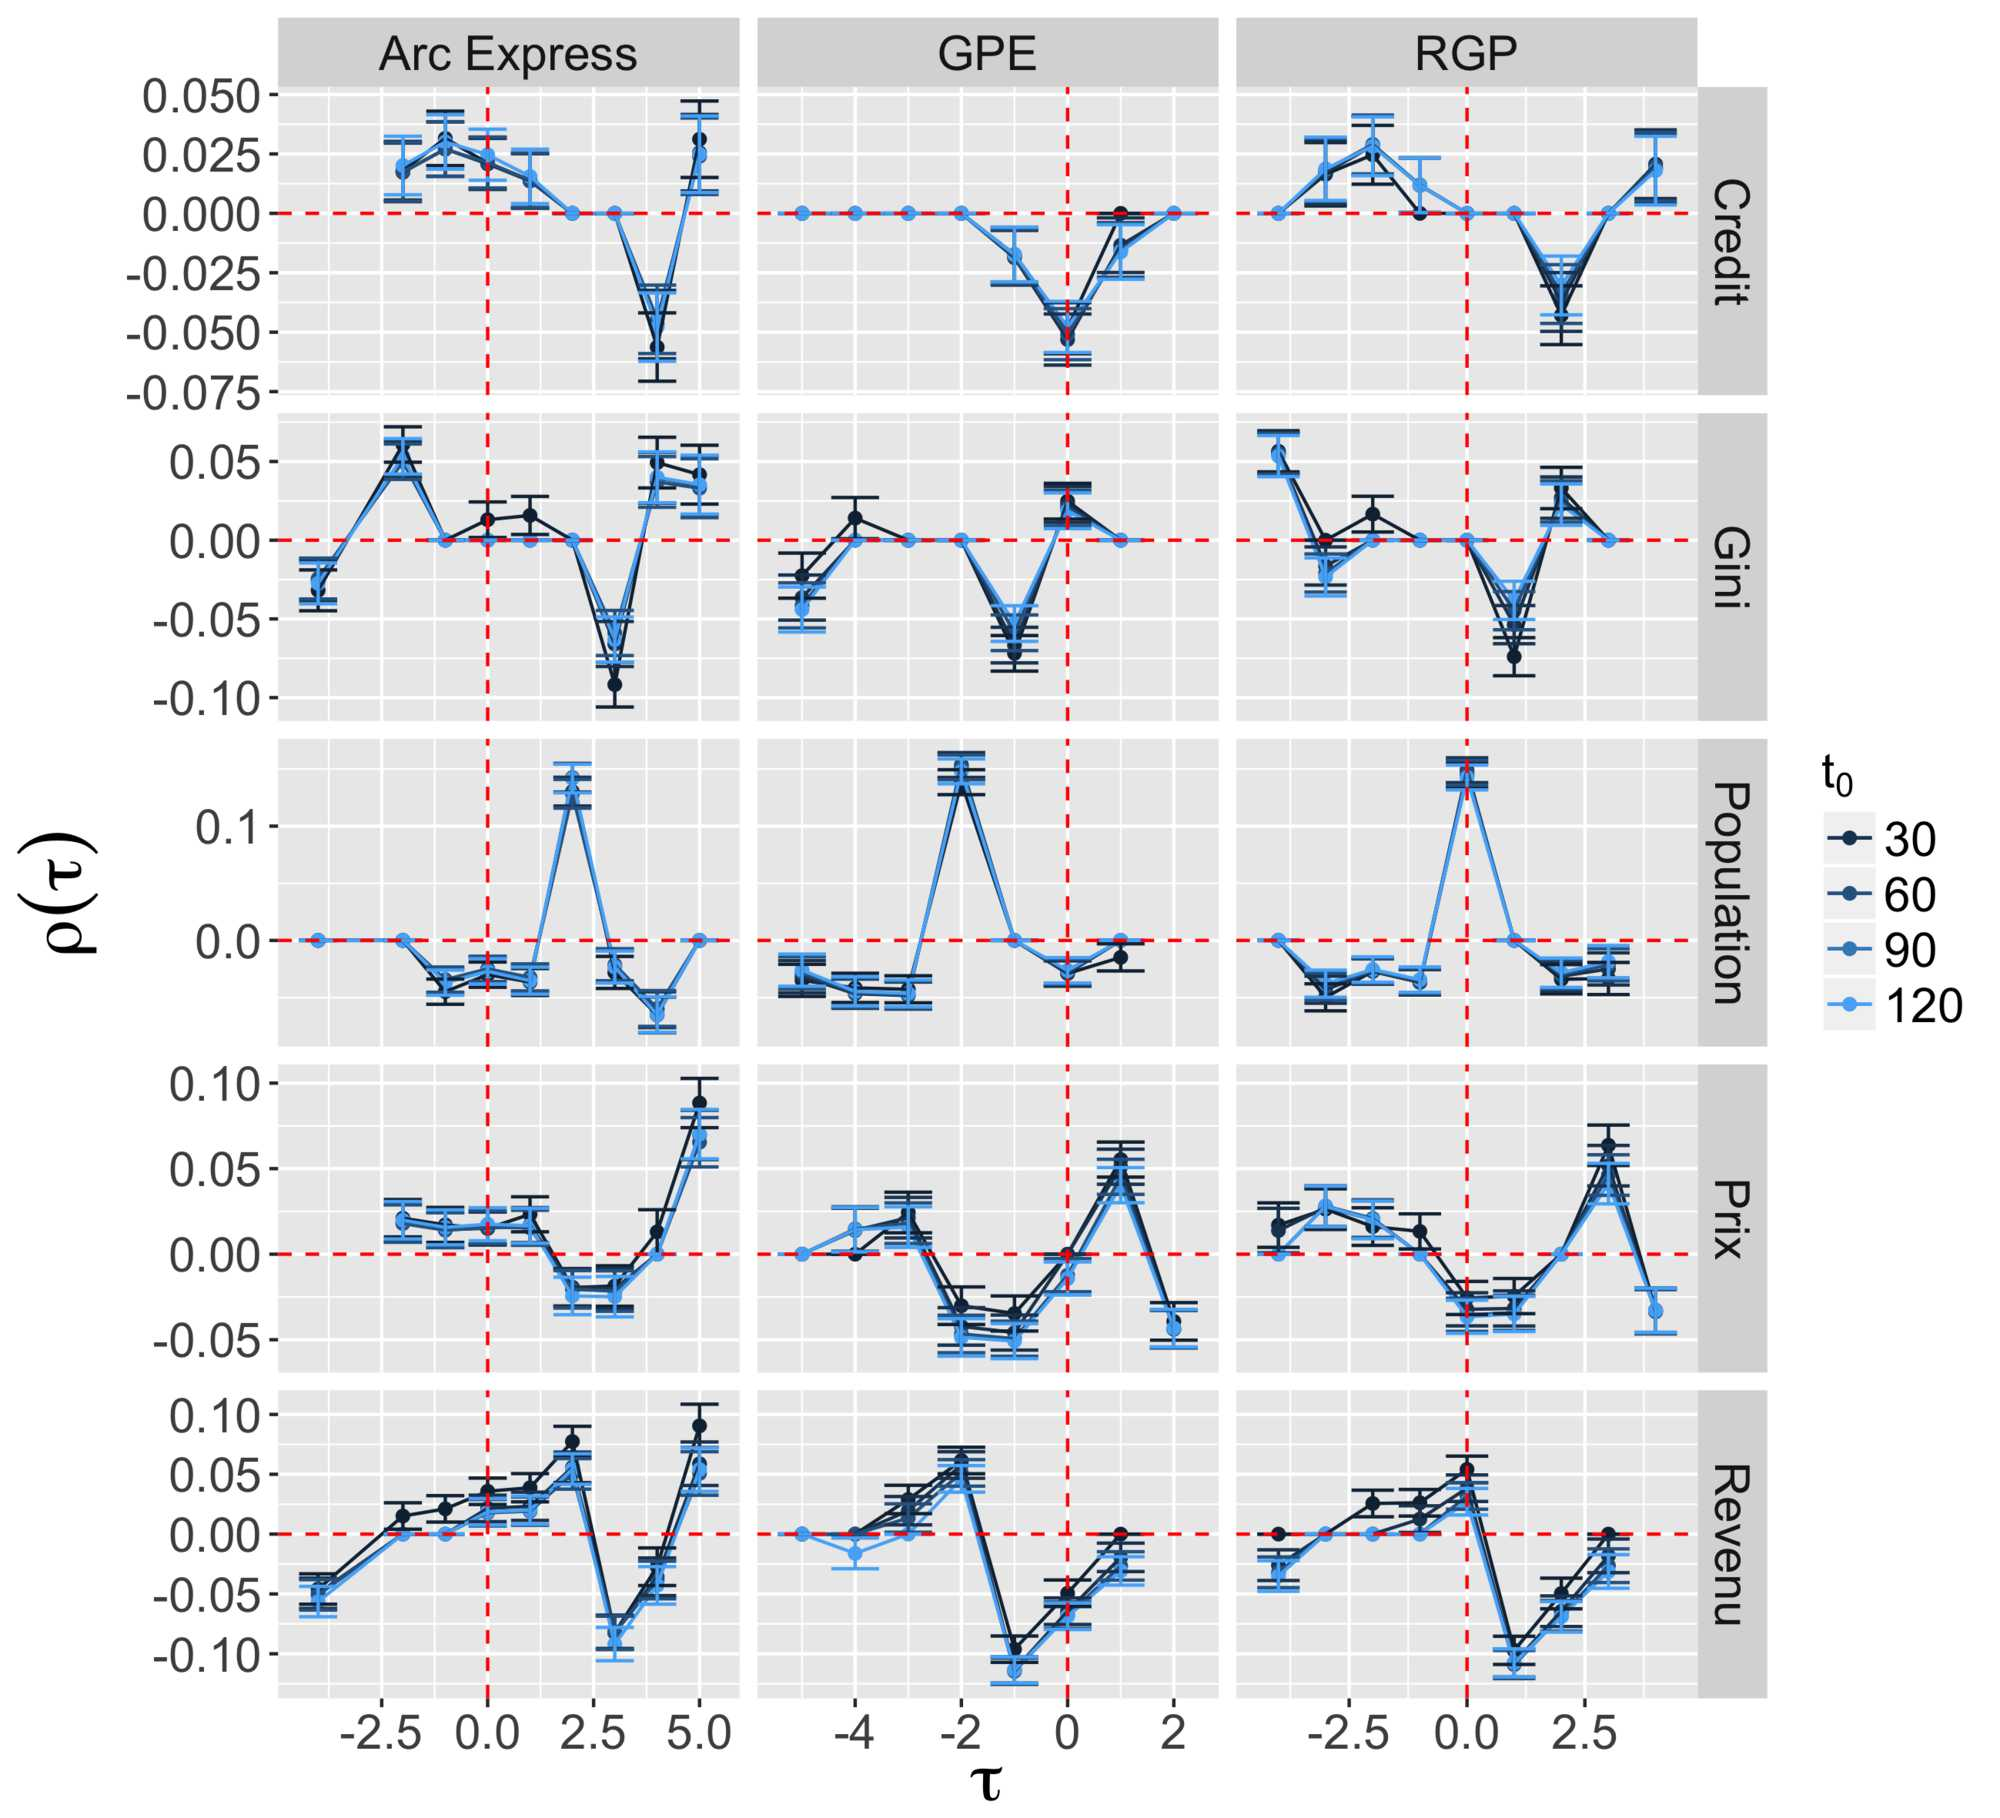
\includegraphics[width=\linewidth]{Figures/Final/1-2-1-fig-casestudies-empiricalres.jpg}
\caption[Empirical lagged correlations between accessibilty gain and territorial variables][Corrélations retardées empiriques entre gain d'accessibilité et variables territoriales]{\textbf{Empirical lagged correlations between accessibilty differential and territorial variables.} Plots show the value of the lagged correlation between differentials of accessibility $\rho(\tau)$ as a function of the lag $\tau$, in terms of average travel time $\Delta T_i$, for each project (in colunms: Arc Express, Grand Paris Express (GPE), Réseau du Grand Paris (RGP)) and the differential of the different socio-economic and real estate variables $\Delta Y_i$ (in rows: values of real estate mortgages (Credit), Average price of real estate transactions (Price), Median income (Income), Gini index for incomes (Gini), Population), for different values of the decay parameter $t_0$. Error bars give the 95\% confidence interval. Dotted red lines are a reading guide: they allow horizontally to check if correlations are significant, and vertically to check the value of the optimal lag. For example, an interpretation of the first row suggests that the older projects have caused a decrease in granted real estae mortgages in Iris hwich accessibility had a positive growth, and that these variables are synchronized for GPE.\label{fig:empiricalres}}{\textbf{Corrélations retardées empiriques entre différentiel d'accessibilité et variables territoriales.} Les graphiques donnent la valeur de la correlation retardée $\rho(\tau)$ en fonction du retard $\tau$, entre le différentiel d'accessibilité en temps de trajet moyen $\Delta T_i$, pour chaque projet (en colonnes : Arc Express, Grand Paris Express (GPE), Réseau du Grand Paris (RGP)) et le différentiel des différentes variables socio-economiques et de transactions immobilières $\Delta Y_i$ (en lignes : valeur des crédits immobiliers (Crédit), Prix moyen des transactions immobilières (Prix), Revenu médian (Revenu), Indice de Gini des revenus (Gini), Population), pour différentes valeurs du paramètre d'atténuation $t_0$. Les barres d'erreur donnent l'intervalle de confiance à 95\%. Les lignes rouges pointillées aident à la lecture : elles permettent horizontalement de voir si les corrélations sont significatives, verticalement de voir la valeur du retard optimal. Par exemple, la lecture de la première ligne suggère que les projets anciens ont causé une baisse des crédits immobilier accordés dans les iris dont l'accessibilité a suivi une croissance positive, et que ces variables sont synchronisées pour le GPE.\label{fig:casestudies:empiricalres}}
\end{figure}
%%%%%%%%%%%%%%%

% disc Thibault : credit devrait pas etre negativement 




\bpar{
We compute for each project, the accessibility differentials $\Delta T_i$ in average travel time from each IRIS, in comparison with the network without the project. Average travel time accessibility is defined as $T_i = \sum_k \exp{-t_{ik}/t_0}$ with $k$ \emph{Communes}, $t_{ik}$ travel time, and $t_0$ a decay parameter. We do not weight here by the population of destination communes, on the contrary to the accessibility $Z_i$ we used previously, to ensure we do not capture any auto-correlation for population or correlations between population and the territorial variables we study. To each project is associated a date\footnote{2006 for \emph{Arc Express}, 2008 for \emph{Réseau du Grand Paris} and 2010 for \emph{Grand Paris Express}}, corresponding roughly to the mature announcement of the project, what remains a bit arbitrary as it is difficult on the one hand to determine precisely as a planning project does not emerge from nothing in one day, and on the other hand it may correspond to different realities of learning about the project by economic agents (we do therefore the limiting but necessary assumption of a diffusion of information for the majority of agents in a time smaller than a year).
}{
Nous calculons pour chaque projet, le différentiel $\Delta T_i$ d'accessibilité temporelle de trajet à partir de chaque IRIS en comparaison à celui dans le réseau sans le projet, où accessibilité temporelle est définie par $T_i = \sum_j \exp{-t_{ij}/t_0}$ avec $j$ communes, $t_{ij}$ temps de trajet, et $t_0$ paramètre d'atténuation. Nous ne pondérons pas ici par la population des communes de destination contrairement à l'accessibilité $Z_i$ utilisée précédemment, pour être certain de ne pas capturer d'auto-corrélation pour la population ou de corrélations entre population et variables territoriales que nous étudions. À chaque projet est associée une date\footnote{2006 pour Arc Express, 2008 pour le Réseau du Grand Paris, 2010 pour le Grand Paris Express.}, correspondant environ à l'année d'annonce mature du projet, restant toutefois arbitraire car difficile d'une part à déterminer précisément, un projet n'émergeant pas d'un coup du jour au lendemain, et d'autre part pouvant correspondre à des réalités différentes d'apprentissage du projet par les différents agents économiques (nous faisons donc l'hypothèse réductrice mais nécessaire d'une diffusion sur la majorité des agents dans un temps inférieur à l'année).
}



\bpar{
The link between accessibility differentials and variations of territorial variables is done through the study of lagged correlations. This method will be developed in details in~\ref{sec:causalityregimes}, but we do not need to enter into technical details here. The idea is the following: if two variables exhibit a strong correlation at a given temporal lag, there is a weak notion of causality, and the variation of the upstream variable may be at the origin of the ones of the variable which is not lagged in time (we use the term weak, since it is of course always possible that correlations are spurious).
}{
Le lien entre différentiels d'accessibilité et variations des variables territoriales est effectué par l'étude des corrélations retardées. Cette méthode sera développée en détails en~\ref{sec:causalityregimes}, mais nous n'avons pas besoin d'entrer dans les détails techniques ici. L'idée est la suivante : si deux variables présentent une forte corrélation avec un certain retard temporel, il y a une notion faible de causalité, les variations de la variable précurseur pouvant être à l'origine de celles de la variable non-décalée dans le temps (on dit faible, car il est toujours possible que les corrélations soient fortuites bien sûr).
}

\bpar{
We study the lagged correlations of $\Delta T_i$ with the variations $\Delta Y_{ij}$ of the following socio-economic variables: population, median income, Gini index for income, average price of real estate transactions and average value of real estate mortgages. Correlation is estimated by lagging accessibility, i.e. by estimating $\rho\left[\Delta T_i(t-\tau),\Delta Y_{i}(t)\right]$. A Fisher test is done for each estimation and the value is set to 0 if it is not significant ($p<0.05$ in a classical manner). The study with generalized accessibility in the sense of Hansen~\cite{hansen1959accessibility} (weighted by populations at destination, or with populations at the origin and employments at destination) has also been conducted but is less interesting as it has a very low sensitivity to the mobility component (network and decay) compared to the variables themselves. It informs therefore only on relations between these and is not presented here.
}{
Nous étudions les corrélations retardées de $\Delta T_i$ avec les variations $\Delta Y_{i}$ des variables socio-économiques suivantes : population, revenu médian, indice de Gini des revenus, prix moyen des transactions immobilières et montant moyen des crédits immobiliers. La corrélation est estimée en retardant l'accessibilité, c'est-à-dire en estimant $\rho\left[\Delta T_i(t-\tau),\Delta Y_{i}(t)\right]$. Un test de Fisher est effectué pour chaque estimation, et la valeur est fixée nulle si celui-ci n'est pas significatif ($p<0.05$ de manière classique). L'étude avec accessibilité généralisée au sens de Hansen~\cite{hansen1959accessibility} (pondérée par les populations à la destination, ou les populations à l'origine et les emplois à la destination) a également été menée mais moins intéressante car très peu sensible à la composante mobilité (réseau et atténuation) par rapport aux variables elle-mêmes, informe uniquement sur des relations entre celles-ci et n'est donc pas présentée ici.
}


\bpar{
We show in figure~\ref{fig:casestudies:empiricalres} the results for all networks and variables. The interpretation can be done the following way: for a variable and a given project, the curve $\rho(\tau)$ can exhibit maxima for a value $\tau_m > 0$ or $\tau_m <0$. This maximal correlation corresponds to a lag giving a ``maximal synchronization'' between the two variables, and the sign of the lag gives the sense of causality between the two variables.
}{
Nous présentons en Fig.~\ref{fig:casestudies:empiricalres} les résultats pour l'ensemble des réseaux et variables. La lecture s'effectue de la façon suivante : pour une variable et un projet donnés, la courbe $\rho(\tau)$ peut présenter des maxima pour une valeur $\tau_m >0$ ou $\tau_m<0$. Cette corrélation maximale correspond à un retard donnant une ``synchronisation maximale'' entre les deux variables, et le signe du retard donne le sens de la causalité entre les deux variables.
}

\bpar{
It is first remarkable to note the presence of significant effects (in the sens of significant correlations and a 95\% confidence interval which does not contains 0) for all variables. Lower values for the parameter $t_0$ give correlations higher in absolute value, unveiling a possible higher importance of local accessibility on territorial dynamics. The behavior of population shows a clearly detached peak corresponding to 2008, what suggests an impact of the older project \emph{Arc Express} on population growth. Under this assumption, the effect of other projects would then be spurious from their proximity in the most important branches. It would imply that areas where they are fundamentally different such as \emph{Plateau de Saclay} are less sensitive to transportation projects, what would confirm the artificial planned aspect of the development of this territory.
}{
Il est remarquable tout d'abord de noter l'existence d'effets significatifs (au sens de corrélations significatives et d'un intervalle de confiance à 95\% ne contenant pas 0) pour l'ensemble des variables. Des valeurs plus basses du paramètre $t_0$ donnent des corrélations plus fortes en valeur absolue, révélant une possible plus grande importance de l'accessibilité locale sur les dynamiques territoriales. Le comportement de la population montre un pic très détaché correspondant à 2008, laissant supposer un impact du plus vieux projet d'Arc Express sur la croissance de la population. Sous cette hypothèse, l'effet des autres projets serait alors fallacieux de par leur proximité dans les grands tronçons. Cela impliquerait d'ailleurs que les zones où ils diffèrent fondamentalement comme le Plateau de Saclay ne soient que très peu sensibles au projet de transport, confirmant l'aspect artificiel planifié du développement de ce territoire.
}

\bpar{
Concerning income, we observe a similar behavior but in a negative way, what would imply a decrease of wealth linked to the increase of accessibility, however accompanied by a decrease of inequalities since the Gini coefficient also presents a negative correlation in positive lags. Finally, real estate prices are as expected driven by the potential arrival of new networks, suggesting a temporal speculation bubble. We demonstrate thus the existence of complex lagged correlation links, that we call causalities in this sense, between territorial dynamics and anticipated dynamics of networks. A finer understanding of implied processes is beyond the scope of this preliminary study and would imply for example qualitative fieldwork or targeted case studies.
}{
Concernant les revenus, on observe un comportement similaire mais négatif, ce qui impliquerait un appauvrissement lié à l'augmentation de l'accessibilité, mais qui semble toutefois s'accompagner d'une baisse des inégalités puisque le coefficient de Gini présente également une corrélation négative dans les retards positifs. Enfin, comme attendu les prix immobiliers sont tirés par l'arrivée potentielle des nouveaux réseaux, effet qui disparait à deux ans pour le Grand Paris Express, suggérant une bulle immobilière passagère dans les quartiers autour des gares. Nous démontrons ainsi l'existence de liens de correlations retardées complexes qu'on nomme causalités en ce sens, entre dynamiques territoriales et dynamiques anticipées des réseaux. Une compréhension plus fine des processus à l'oeuvre est au delà de la portée de cet étude préliminaire, car supposerait par exemple des études de terrain qualitatives ou des études de cas ciblées.
}




\bpar{
This study suggests potential effects of the modification of accessibility due to Greater Paris projects, since some effects that were revealed can be linked to planning policing that also anticipate the new network. We thus suggest an effective existence of processes implying an effect of the network on territories, since most optimal lags are positive.
}{
Cette étude suggère des effets potentiels de la modification d'accessibilité due au projets du Grand Paris, puisque certains effets révélés peuvent être liés à des politiques d'aménagement anticipant également le nouveau réseau. On suggère ainsi une existence réelle des processus d'effet du réseau sur les territoires, puisque la majorité des retards optimaux sont positifs.
}












%-------------------------


%%%%%%%%%%%%%%%%%%%%%%%%
%\subsection[Pearl River Delta][Le Delta de la Rivière des Perles]{Pearl River Delta: new urban regimes and mega-city regions}{Le Delta de la Rivière des Perles : nouveaux régimes urbains et Mega-région urbaine}
\subsection{Pearl River Delta}{Le Delta de la Rivière des Perles}


\bpar{
We now switch the geographical region, the urban structure, and the time period, in order to describe an other relevant case study in China. The extended Parisian region can be read as a consistent entity\footnote{\cite{gilli2005bassin} recalls the importance of the hinterland of Bassin Parisien and the importance of not considerating the hypercenter in an isolated way, and thus considerate the MCR which includes a certain number of important urban centers at one hour of Paris: Chartres, Orléans, Rouen, Reims and Lille thanks to High Speed Lines.}: it would be a \emph{mega-city region}, concept that we will now define and develop for the particular instance of Peral River Delta.
}{
Nous changeons à présent de région géographique, de structure urbaine, de période temporelle, pour évoquer un autre cas d'étude pertinent en Chine. La région parisienne étendue peut être lue comme un ensemble cohérent\footnote{\cite{gilli2005bassin} rappelle l'importance de l'hinterland du Bassin Parisien et l'importance de ne pas considérer l'hypercentre de manière isolée, et considérer ainsi la MCR qui inclut un certain nombre de centres urbains importants à une heure de Paris : Chartres, Orléans, Rouen, Reims et Lille grâce à la grande vitesse.} : il s'agirait d'une \emph{méga-région urbaine}, concept que nous allons à présent définir et développer pour l'instance particulière du Delta de la Rivière des Perles.
}


% \cite{weissberg1997delta} ref fr prd
% \cite{lin1999transportation} panyu district developpement


\subsubsection{New urban regimes and mega-city regions}{Nouveaux régimes urbains et méga-régions urbaines}

\bpar{
The notion of megalopolis has been introduced by~\cite{gottmann1961megalopolis} to designate the emergence of urban agglomerates at a scale that did not exist before. It is at the origin of the concept of \emph{Mega-city Region} (MCR) which was consecrated by~\cite{hall2006polycentric}. For the European case, they unveil assemblies of metropolis that are strongly connected regarding mobility flows, connections between companies, which form what they call polycentric \emph{Mega-city Regions} (for example Randstad in Netherlands, the Rhine-Rhur region in Germany). Their characteristics are a certain geographical proximity of centers, a strong integration through flows, and a certain level of polycentrism. It consists in an urban form that did not exist before, which emergence seems linked to globalization processes.
}{
La notion de megalopolis a été introduite par~\cite{gottmann1961megalopolis} pour désigner l'émergence d'agglomérats urbains à une échelle non-existante auparavant. Elle est à l'origine du concept de \emph{Mega-city Region} (MCR) consacré par~\cite{hall2006polycentric}. Sur le cas Européen, ils dégagent des ensembles de métropoles fortement connectées par rapport aux flux de mobilité, aux connections entre entreprises, qui forment ce qu'il appellent des \emph{Mega-city Regions} polycentriques (par exemple la Randstad aux Pays-bas, la région Rhin-Ruhr en Allemagne). Les caractéristiques sont une certaine proximité géographique des centres, une forte intégration par les flux, et un certain niveau de polycentrisme. Il s'agit d'une forme urbaine inédite par le passé, dont l'émergence semble liée aux processus de globalisation.
}

%% TODO :
% Idees :
%  1) again the concept of transition : to what extent can we formulate a generic meta model of the transmondyn transitions ? find these general regularities ? test and compare all models computationally ?
%  2) we use the term "certain" proximity and level of polycentrism (by the way how is it measured ?) -> todo a study à-la-Cottineau but on MCR's, possibly at multiple scales, using different dimensions ? (may rejoin endogenous characterisation of MCR's through bottom-up morphological Le Nechet's characterizations...)



\bpar{
This concept is even more relevant with the recent emergence of new types of urbanization, in particular through the accelerated urbanization in countries with a strong economic growth and undergoing a very rapid mutation such as China~\cite{swerts2015megacities}.
}{
Ce concept est toujours plus d'actualité avec l'apparition récente de nouveaux types d'urbanisation, notamment par l'urbanisation accélérée dans des pays à forte croissance économique et en mutation très rapide comme la Chine~\cite{swerts2015megacities}.
}




\bpar{
The second case that we develop here enters this category: Pearl River Delta (PRD) is one of the classical illustrations of the structure of a strongly polycentric MCR. Historically initially only composed by Guangzhou, the development of Hong-Kong and the establishment of Special Economic Zones (SEZ) in the context of opening policies by \noun{Deng Xiaoping}, lead to an extremly rapid development of Shenzhen, and in a less proportion of Zhuhai\footnote{Shenzhen and Zhuhai were among the first Special Economic Zones, created in 1979 to attract foreign investments in these areas with flexible economic rules. The development model of Zhuhai was different of Shenzhen, since heavy industry was forbidden.}. Guangdong province in which PRD is fully located has currently the highest regional GDP within China, and the MCR contains a population of around 60 millions (estimations strongly fluctuate depending on the definition of the MCR which is taken, and the inclusion of the floating population). The phenomenon of migrations from rural areas is highly present in the region and a city such as Dongguan has for example based its economy on factories employing these migrant workers.
}{
Le second cas que nous développons ici rentre dans cette catégorie : le Delta de la Rivière des Perles (PRD) est une des illustrations classiques de la structure d'une MCR fortement polycentrique. Historiquement initialement composé de Guangzhou uniquement, le développement de Hong-Kong puis la mise en place des Zones Économiques Spéciales (ZES) dans le cadre des politiques d'ouverture de \noun{Deng Xioaping}, a conduit à un développement extrêmement rapide de Shenzhen, et dans une moindre mesure de Zhuhai\footnote{Shenzhen et Zhuhai ont été parmi les premières Zones Économiques Spéciales, instaurées en 1979 pour attirer les investissements étrangers dans ces zones aux règles économiques flexibles. Le modèle de développement de Zhuhai a été différent de celui de Shenzhen, puisque l'industrie lourde y était interdite.}. La province du Guangdong dans lequel le PRD se situe intégralement a actuellement le plus fort PIB régional de Chine, et la MCR regroupe une population d'environ 60 millions (les estimations fluctuant fortement selon la définition prise de la MCR et la prise en compte de la population flottante). Le phénomène de migration des campagnes est très présent dans la région et une ville comme Dongguan a par exemple basé son économie sur des manufactures employant ces travailleurs migrants.
}


\subsubsection{Governance of the mega-city region}{Gouvernance de la méga-région urbaine}

\bpar{
\cite{Ye2014200} analyzes the actions of metropolitan governance at the scale of centers of the MCR, and more particularly how municipalities of Guangzhou and Foshan have progressively increased their cooperation to form an integrated metropolitan area, what can thus strongly influence the development of transportation for example and allowing the construction of a connected network. A strong tension between bottom-up processes, and a state control which is relatively strong in China, which originates from the Central State, to the province government and local government, has allowed the emergence of such a structure. The competition with other cities in the MCR remains strong, and the logic of integration (in the sense of articulation between the different centers, of interactions and of flows between these) of the MCR is only partly guided by the region. The particular nature of SEZ of Shenzhen and Zhuhai, linked to the privileged relations with the Special Administrative Zones of Hong-Kong and Macao, which have returned to the Popular Republic only at the end of the last millenium and keep a certain level of independence in terms of governance, complicates even more the relations between actors within the region. The issue of a correspondence between some levels of governance and urban processes is a tricky one: \cite{liao2017ouverture} interprets the progressive transfers of economic initiatives from the central power to local authorities as a form of a multi-level governance.
}{
\cite{Ye2014200} analyse les actions de gouvernance métropolitaine à l'échelle des centres de la MCR, et plus particulièrement comment les communes de Guangzhou et Foshan ont progressivement accru leur coopération pour former une zone métropolitaine intégrée, pouvant ainsi fortement influencer le développement des transports par exemple et permettant la mise en place d'un réseau connecté. Une forte tension entre des processus émergents par le bas, et un dirigisme d'état relativement fort en Chine, se répercutant de l'État central, au gouvernement provincial jusqu'aux gouvernements locaux, a permis la mise en place d'une telle structure. La compétition avec les autres villes de la MCR reste très forte, et la logique d'intégration (au sens d'articulation entre les différents centres, d'interactions et de flux entre ceux-ci) de la MCR est seulement partiellement guidée par la région. La nature particulière des ZES de Shenzhen et Zhuhai, liée aux relations privilégiées avec les Zones Administratives Spéciales de Hong-Kong et Macao, qui n'ont été réintégrées à la République Populaire qu'à la fin du millénaire et conservent un certain niveau d'indépendance en termes de gouvernance, complique encore les jeux d'acteurs au sein de la région. La question de la correspondance entre certains niveaux de gouvernance et des processus urbains est épineuse : \cite{liao2017ouverture} interprète les transferts progressifs des initiatives économiques du pouvoir central vers les autorités locales comme une forme de gouvernance multi-niveaux.
}

% Note (trad) : strange (partisan ?) formulation of the status of SAZ ?

%\comment{district panyu}
%  Cette propriété complexe ne couvre cependant pas tous les domaines ni tous les niveaux : il n'existe pas d'autorité d'organisation des transports au niveau de la MCR, et chaque commune gère indépendamment le réseau local, tandis que les connections entre villes sont assurées par le réseau de train national. Cela confirme d'une part un certain niveau de concurrence entre les différents centres de la MCR, et induit une structure urbaine particulière, de très fortes densités pouvant alterner avec des zones rurales très peu développées ni accessibles. La présence d'une ligne de transport en commun lourd influence fortement le développement : \cite{lin1999transportation} étudie l'exemple du district Panyu de Guangzhou, qui a connu au tournant du millénaire un développement exponentiel conjointement avec la construction d'une ligne de métro spécifique, comme une stratégie de la ville de Guangzhou pour étendre son emprise au sud.


\subsubsection{Transportation Governance}{Gouvernance des transports}

%%%%%%%%%%
%% -- TRAD --
%%%%%s%%%%%

\bpar{
In the frame of transportation within the MCR, there is no specific authority at this scale for the organization of transportation (but indeed entities at the level of the State, of the province and of municipalities), and each municipality manages independently the local network, whereas the connections between cities are ensured by the national train network. This leads to particular situations in which some areas have a very low accessibility, with a very strong heterogeneity locally. Therefore, the southern part of the city of Guangzhou which constitutes a direct access to the sea, is geographically closer to the center of Zhongshan, but a direct link by public transport is difficult to imagine, whereas the area is well linked to the center of Guangzhou by the metro line. A similar situation can be observed at the terminus of line 11 in Shenzhen, for the neighbor district of Dongguan, the latest having a very low accessibility by public transport.
}{
Dans le cadre des transports pour la MCR, il n'existe pas d'autorité spécifique à cette échelle pour l'organisation des transports (mais bien des entités au niveau de l'État, de la province et des communes), et chaque commune gère indépendamment le réseau local, tandis que les connections entre villes sont assurées par le réseau de train national. Cela conduit à des situations particulières dans lesquelles des zones se retrouveront très enclavées, avec une hétérogénéité très forte localement. Ainsi, la pointe sud de la ville de Guangzhou qui sert d'accès direct à la mer, est plus proche géographiquement du centre de Zhongshan, mais un lien direct par transports en commun est difficile à envisager, alors que la zone est bien reliée au centre de Guangzhou par la ligne de métro. Une situation similaire s'observe au terminus de la ligne 11 de Shenzhen, pour le quartier limitrophe de Dongguan, ce dernier étant très peu accessible en transports en commun\footnote{Voir la carte~\ref{fig:casestudies:prd} pour les localisations, celle-ci donnant par ailleurs les accessibilités par réseau routier.}. Cette situation serait cependant transitoire, étant donné les infrastructures déjà en construction et celles planifiées sur un plus long terme : le métro de Shenzhen, qui couvre aujourd'hui 285km, est planifié pour atteindre jusqu'à 30 lignes et une longueur d'environ 1100km\footnote{A titre de comparaison, le réseau Transilien a une longueur avoisinant les 1300km en incluant les lignes RER, ce qui pourrait les rendre comparable, mais il faut garder à l'esprit que l'Ile-de-France a une surface de 12000km$^2$ contre 2000km$^2$ pour Shenzhen. Cela implique pour Shenzhen une densité de desserte bien plus haute, correspondant aux zones de fortes densité urbaine, si bien que le plan prévoit 70\% de transit par métro à l'horizon 2030.} en 2030 comme déclaré par le plan officiel de la ville~\cite{shenzhen2016plan}. Il est clair que ces développements suivent pour la majorité un développement urbain existant, une question cruciale est la volonté et la capacité à contenir l'étalement urbain et structurer les futurs développements autour de ce nouveau réseau, dans l'esprit d'une intégration volontaire entre urbanisme et transport de type \emph{Transit Oriented Development} que nous avons introduit précédemment. Différents terminus seront connectés au metro de Dongguan, et de nouvelles lignes intercités structureront les déplacements de plus longue portée, ce qui fera du Delta dans un horizon temporel proche une MCR relativement bien intégrée en termes de transports en communs. Pour se donner une idée du développement du réseau dans les années à venir, la Table~\ref{tab:casestudies:stats} donne la taille des réseaux planifiés dans les différentes villes d'ici 2030.
}

%%%%%%%%%%%%%
\begin{table}
\caption[Public transportation in Pearl River Delta][Transports en commun dans le Delta de la Rivière des Perles]{\textbf{Public transportation in Pearl River Delta.}\label{tab:casestudies:stats}}{\textbf{Transports en commun dans le Delta de la Rivière des Perles.} Nous donnons les populations en 2010 issues de \cite{yearbook2013guangdong}. Les kilométrages sont issus des différents documents de planification pour les metros de Guangzhou~\cite{guangzhou2016metro}, Shenzhen~\cite{shenzhen2016plan} et Dongguan~\cite{dongguan2017ditie} et pour le tramway de Zhuhai~\cite{zhuhai2016tram}. Zhongshan n'est pas incluse car exploite un système de bus en site propre mais pas d'infrastructure lourde.\label{tab:casestudies:stats}}
\begin{tabular}{|c|c|c|c|}\hline
	Ville & Population & Réseau 2016 & Réseau 2030 \\\hline
	Guangzhou - Foshan & 18.9 Mio & 390km & 800km \\\hline
	Shenzhen & 10.4Mio & 286km & 1124km \\\hline
	Dongguan & 8.2Mio & 38km & 195km \\\hline
	Zhuhai (Tramway) & 1.6Mio & 10km & 173km \\\hline
\end{tabular}	
\end{table}
%%%%%%%%%%%%%

%\comment[CL]{D’où viennent ces chiffres? Je ne connait pas les chiffres exactes des autres villes mais je suis sure des chiffres de Zhuhai car j’ai récemment travaillé dessous. La population permanent de Zhuhai en 2010 selon les chiffre officielle était de: 1,562,530 (hukou pop.: 1,048,398; Pop. Flottante: 514,132) * www.stats-zh.gov.cn}

% Zhongshan : specialisation eco locale.


\subsubsection{Impact of the Zhuhai-Hong-Kong-Macao bridge}{Impact du pont Zhuhai-Hong-Kong-Macao}

Un projet majeur d'infrastructure de transport dans la région est le pont-tunnel fermant l'embouchure du Delta, reliant Zhuhai et Macao à Hong-Kong (HZMB). La longueur de la traversée est de 36.5km, ce qui en fait un ouvrage d'art exceptionnel~\cite{hussain2011hong}. L'ouverture au traffic a été retardée de plusieurs années et est prévue finalement en 2018\footnote{Voir le site officiel à \url{http://www.hzmb.org/cn/default.asp}.}. \cite{zhou2016medium} montre que les changements de motifs d'accessibilité attendus pour l'Ouest du Delta sont relativement forts, et ceux-ci peuvent potentiellement induire de fortes bifurcations dans les trajectoires des villes. La nécessité du projet est défendue par les différents porteurs du projet (Province du Guangdong, Région Administrative Spéciale de Hong-Kong, Région Administrative Spéciale de Macao) par des arguments de fort bénéfice économique dans le cadre des politiques d'ouverture, ainsi que par un bénéfice social pour l'Ouest notamment. Par exemple, Zhuhai se positionne comme un nouveau pivot entre Hong-Kong et l'ouest. L'équilibrage d'accessibilité, au sens de la diminution des inégalités spatiales d'accessibilité, s'opère cependant pour le mode routier uniquement, ce qui conduit à questionner ses impacts potentiels : d'une part l'accès à l'automobile reste réservé à une partie de la population seulement, d'autre part les effets négatifs de la congestion peuvent rapidement modérer les gains d'accessibilité. Ces gains d'accessibilité sont cartographiés suivant la même méthode que précédemment, et montrés avec l'accessibilité $Z_i$ elle-même en Fig.~\ref{fig:casestudies:prd}.


% Un projet iconique d'infrastructure de transport dans la région est le pont fermant l'embouchure du Delta, reliant Zhuhai et Macao à Hong-Kong. En réalité un Pont-tunnel, celui-ci fait une cinquantaine de kilomètres, en faisant le plus long du monde. L'ouverture au traffic a été retardée de plusieurs années et est prévue pour fin 2017. Le changement de motifs d'accessibilité peut potentiellement induire de fortes bifurcations dans les trajectoires des villes. La ville de Zhuhai oriente son développement urbain et économique en tirant profit de cette nouvelle liaison : implantation d'une High-tech zone accueillant des nouvelles entreprises du numériques avec l'idée d'imiter Shenzhen dans son statut de ``Silicon Valley'' chinoise, projet d'infrastructures (transport, parc des expositions) et immobiliers dans des nouveaux quartiers bordant Macao et donc l'accès à Hong-Kong par le pont. Les processus de gouvernance jouent encore un rôle dans les dynamiques socio-économiques, puisque pour le court terme et les dynamiques d'emplois, les résidents de Zhuhai disposent d'un statut unique leur permettant de se rendre librement à Hong-Kong et Macao (ce que ne peuvent pas faire les résidents de Shenzhen pour Hong-Kong par exemple). L'impact direct du pont sur l'accessibilité régionale est clair et montre un fort rééquilibrage entre l'Est et l'Ouest de la région.
% \cite{hou2011transport}
% On peut spéculer que ce gain d'accessibilité peut permettre à Zhuhai de maintenir une trajectoire de fort développement, et il est possible que la trajectoire de villes plus à l'Ouest comme Jiangmen voient leur forme qualitativement changée, témoignant d'une bifurcation dans le système urbain local.

%%%%%%%%%%%%%%
\begin{figure}
	%\includegraphics[width=0.49\linewidth]{Figures/CaseStudies/accessp_withbridge_prd.png}
	%\includegraphics[width=0.49\linewidth]{Figures/CaseStudies/accesspdiff_prd.png}
	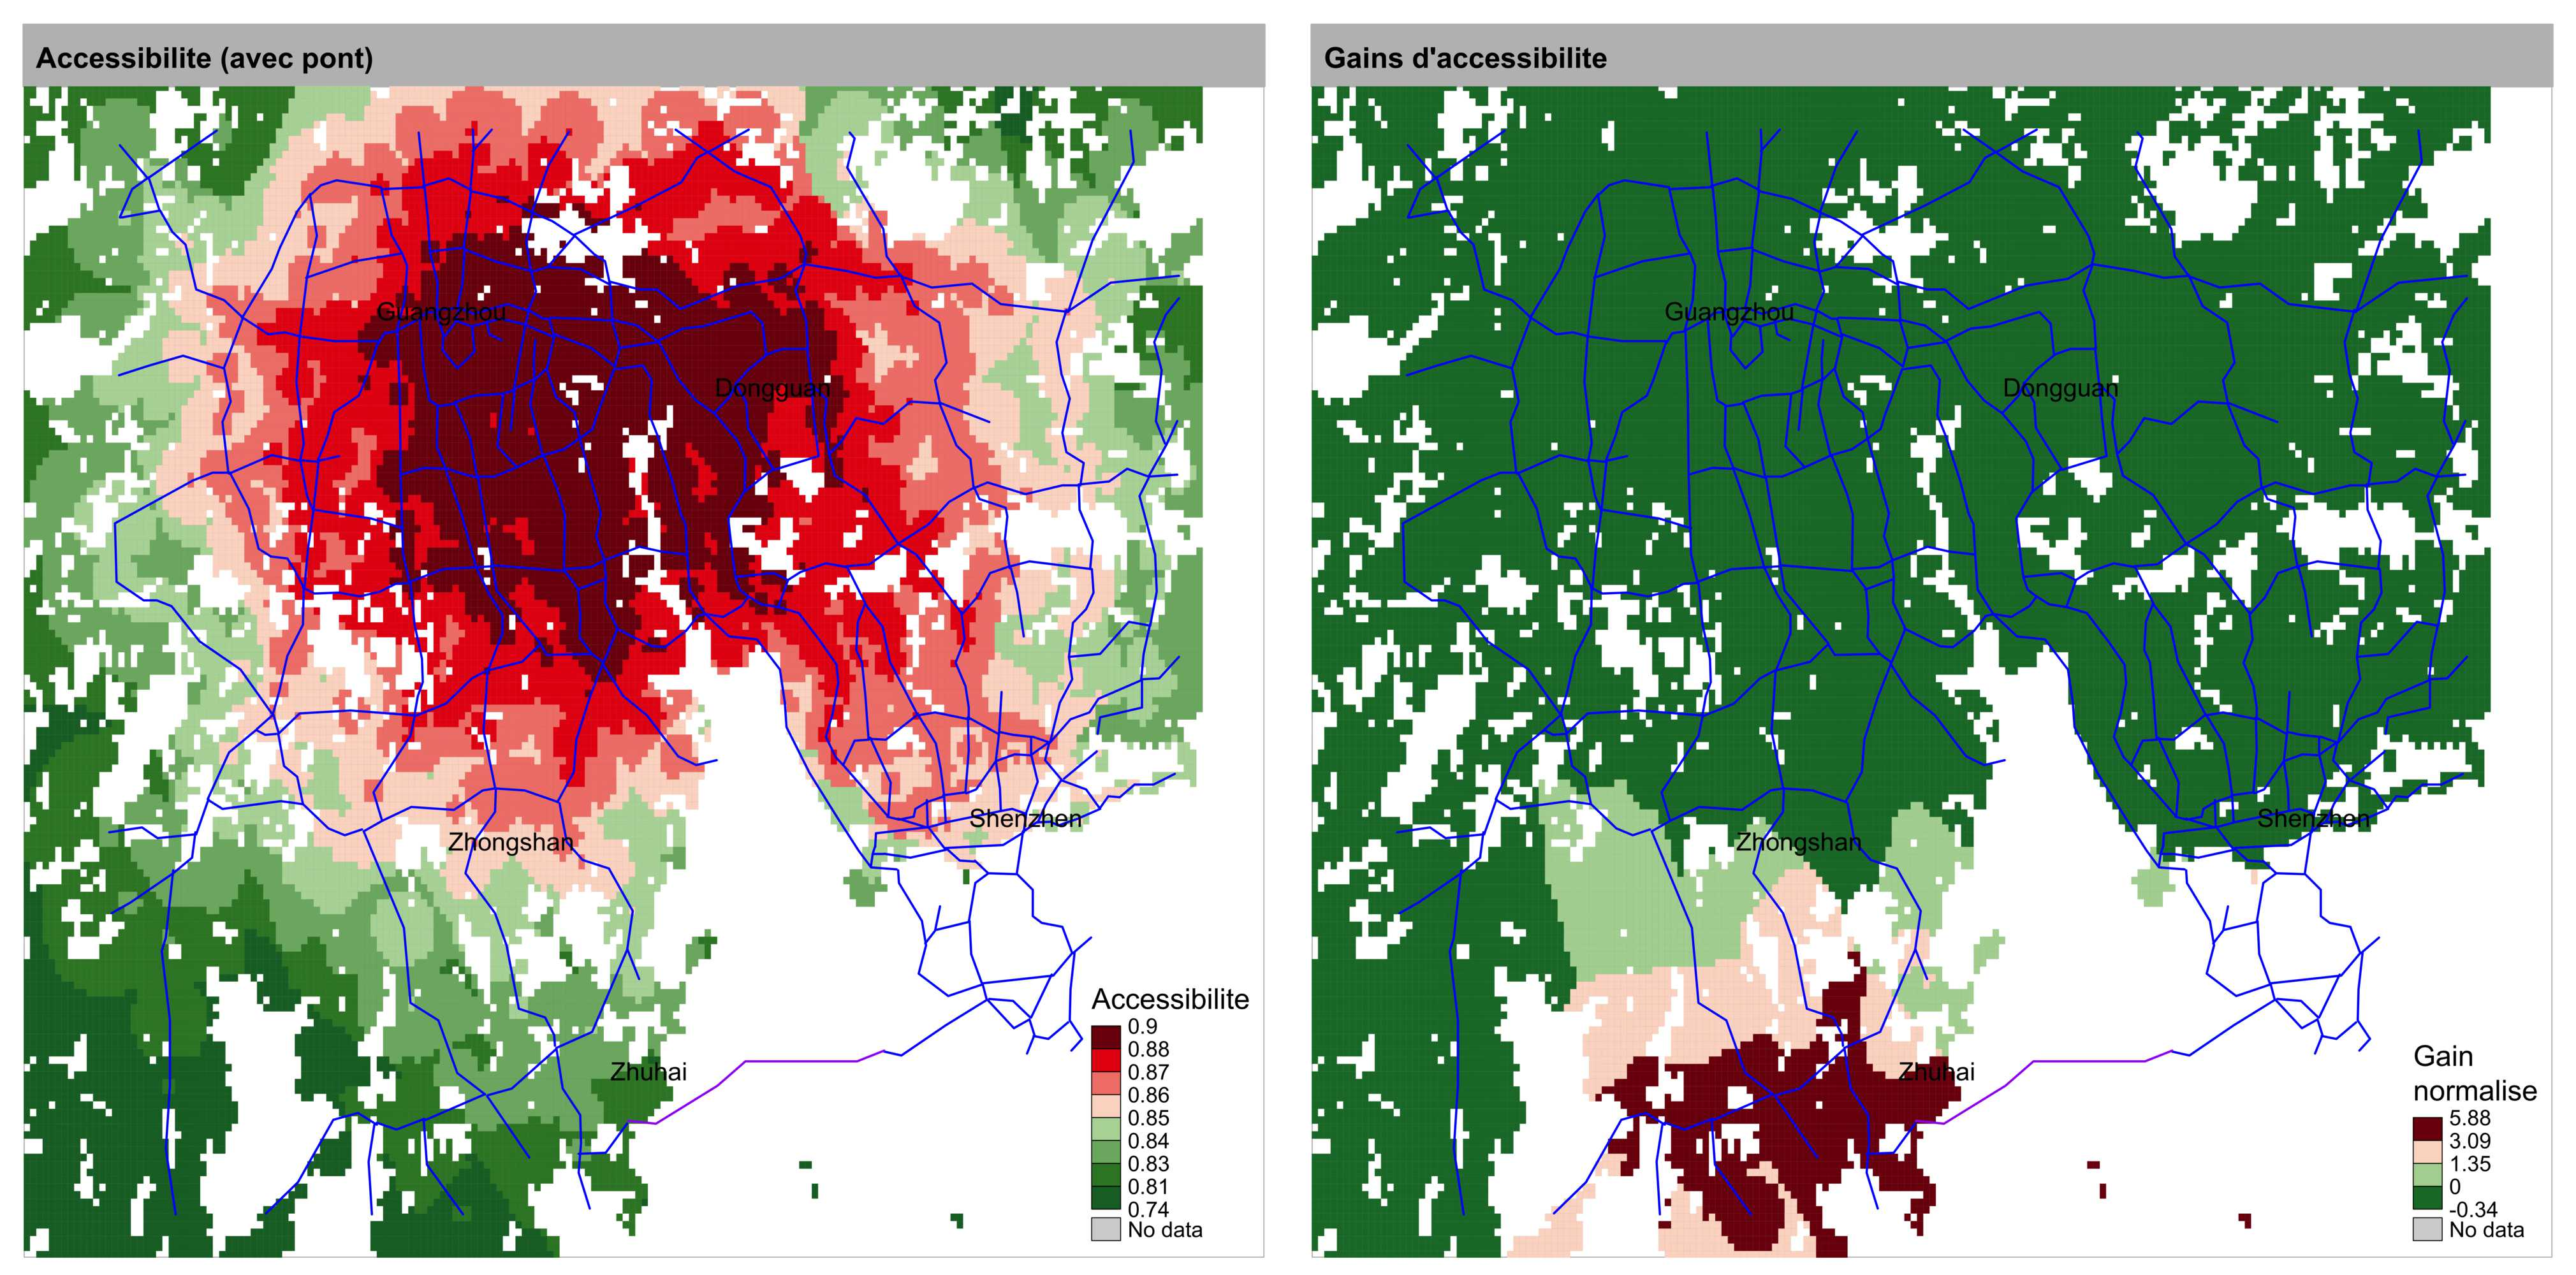
\includegraphics[width=\linewidth]{Figures/Final/1-2-1-fig-casestudies-prd.jpg}
	\caption[Accessibility gain thanks to HZMB][Gain d'accessibilité permis par le pont Hong-Kong-Zhuhai-Macao]{\textbf{Accessibility gain thanks to HZMB.}\label{fig:casestudies:prd}}{\textbf{Gain d'accessibilité permis par le HZMB dans le Delta de la Rivière des Perles, pour le territoire de Chine continentale.} (\textit{Gauche}) Accessibilité à la population $Z_i$ ; (\textit{Droite}) Gains normalisés d'accessibilité. La population de Hong-Kong est prise en compte dans les points de destination. Le réseau autoroutier (2017) est cartographié en bleu et le nouveau lien du pont en violet.\label{fig:casestudies:prd}}
\end{figure}
%%%%%%%%%%%%


Les impacts à moyen et long terme du pont sont ainsi difficiles à estimer. \cite{wu2012impact} trouve des motifs similaires à ceux que nous estimons, c'est-à-dire un bénéfice significatif pour Zhuhai (et Hong-Kong que nous n'avons pas pris en compte), ainsi que des effets immédiats de modification de traffic et des impacts économiques liés au péage ou à l'accroissement du tourisme. Ils postulent surtout la position de Zhuhai-Macao comme un nouveau pivot dans la région. Si cela est vérifiable immédiatement en termes de centralité et d'accessibilité, il n'est pas dit que cette nouvelle position influence particulièrement la trajectoire socio-économique de Zhuhai. Un accompagnement politique particulier passant par une collaboration accrue entre Hong-Kong, Zhuhai et Macao sera importante~\cite{zhou2016medium}. Des effets économiques immédiats sont attendus, comme une augmentation des résidents de Zhuhai travaillant à Hong-Kong (les habitants de Zhuhai sont les seuls de la région à bénéficier d'une carte spéciale leur permettant de se rendre régulièrement dans les Zones Administratives Spéciales\footnote{Source : sortie de terrain du 06/11/2016 avec C. Losavio (voir~\ref{app:sec:qualitative}).}), mais le contraire, comme des investissements de Hong-Kong vers l'ouest du Delta n'ont pas de raison d'être systématiques : le premier cas prolonge la dynamique déjà existante avec Macao, le second est à construire en grande partie. Ainsi, cet exemple est un cas typique de notre problématique générale.


\subsubsection{Perspectives}{Perspectives}

\bpar{}{
Une piste d'exploration passant par la modélisation consiste à poser le problème différemment et de chercher comprendre la dynamique du système métropolitain de manière intégrée, c'est-à-dire comme un système territorial en notre sens, dans lequel le couplage fort entre territoire et réseau est opéré par une ontologie propre des entités de gouvernance. Celle-ci sera l'objet de la section~\ref{sec:lutecia}.
}

\bpar{}{
Cette deuxième étude plus brève nous a permis de mettre en valeur une structure de gouvernance fondamentalement différente, mais la même idée d'un projet de transport considérable modifiant profondément les motifs d'accessibilité. Les attentes des acteurs quant aux mutations territoriales potentiellement induites sont comparables au sens qu'une forte attente est mise dans le projet.
}

%-------------------------


%%%%%%%%%%%%%%%%%%%%%%%%
\subsection{Comparability of case studies}{Comparabilité des études de cas}


Nous avons étudié ici deux cas de développement métropolitain et de projets d'infrastructures dans leurs cadres. La possibilité de transfert des modèles urbains (comme le TOD), au sens de l'applicabilité de cadres génériques à des contextes géographiques différents, est généralement délicate. La synthèse de conclusions empiriques issus de cas d'étude très éloignés l'est également.


La particularité Est-asiatique a déjà été montrée pour la structure économique, et comment celle-ci ne peut être interprétée de manière simple par une séparation des processus microscopiques et macroscopiques comme certaines lectures rapides et idéologiquement orientée ont pu le faire, comme la vision de la Banque Mondiale~\cite{amsden1994isn}. La comparabilité de systèmes urbains est une question ouverte au centre des enjeux de la Théorie Evolutive Urbaine. Celle-ci est liée au caractère ergodique de ces systèmes : l'hypothèse d'ergodicité postule que la trajectoire d'une ville dans le temps capture l'ensemble des états urbains possibles, et ainsi que les différentes villes sont différentes manifestations du même processus stochastique à différentes périodes. Dans ce cas, un ensemble de villes permettrait de se faire une idée des trajectoires temporelles. Intuitivement ce n'est pas le cas, et les systèmes urbains seraient plutôt non-ergodiques~\cite{pumain2012urban}. Empiriquement, cette non-correspondance entre statistiques globales et dynamiques individuelles des villes est montrée pour des données de traffic par~\cite{2017arXiv171009559D}. Ainsi il s'agira de rester prudent pour la généralisation des conclusions, autant empiriques que théoriques, ou issues de la modélisation.


% On peut noter toutefois certains aspects généraux qui se dégagent de ces deux études de cas.

%\comment[FL]{cela semble hors sujet. plutot fin chap 2. dans chap 1 on parle des processus, pas des modeles.}[en fait non si on parle des modeles urbains comme le tod.]

%\comment[JR]{ouverture sur le perspectivisme : besoin de multiples cas pour esperer avoir des modeles generiques (cf multilevel comparison of large urban systems); possibilite du transfert de modeles (cf Q a conf Medium)}




\stars


Nous avons donc vu dans cette section, à partir de deux études de cas très différentes, mais ayant le point commun de présenter des projets significatifs d'infrastructures de transport, que les impacts immédiats de celles-ci en termes d'accessibilité peuvent être conséquents, mais qu'il est compliqué d'associer ces gains à de possibles mutations futures. Nous commençons à entrevoir la difficulté de caractériser la co-évolution.


Nous allons dans la section suivante encore diversifier nos exemples, à partir d'observations de terrain, et donc selon un point de vue plus subjectif et complémentaire.



\stars









